\cs{Group Finder Algorithm}
\begin{quotation}
\noindent{\rule{\linewidth}{0.5pt}}
--  " Le plus simple serait que tout se fasse le plus simplement possible "\\
\textit{Inconnu}\\
\noindent{\rule{\linewidth}{0.5pt}}
\end{quotation}
\minitoc

\fs{Introduction}
Les grands relevés du ciel sont utilisés de manière courante dans la recherche en astronomie et prennent de plus en plus de place
dans la façon de travailler des chercheurs, surtout sur l'étude des structures des galaxies aux grandes échelles dans l'Univers. Un
des plus fameux "surveys", est le SDSS (Sloan Digital Sky Survey) qui permet d'avoir accès aux spectres et aux mesures
photométriques de presque un million de galaxies sur la voûte céleste. Ces données sont mises à jour annuellement et ne cessent
donc de s'enrichir. Cette abondance de données a abouti à de nombreuses études qui ont permis de mesurer l'évolution des propriétés
des galaxies (comme la couleur, le contenu en gaz, la morphologie, l'âge, l'abondance en métaux...) avec leur \emph{masse en
étoiles}, leurs \emph{environnements global} (avec leur groupe parent) et \emph{local} (distance au centre du groupe parent). Ces
propriétés découlent de processus physiques qui dépendent fortement de la quantification des environnements des galaxies. Il est
donc important de pouvoir réaliser cette quantification de manière optimale afin de comprendre au mieux ces processus physiques.
C'est alors le but de ce stage: créer un programme qui permet de regrouper au mieux les galaxies du SDSS.

Mais ce regroupement n'est pas des plus simples à réaliser. Beaucoup d'effets sont à prendre en compte afin de quantifier les
environnements et vont faire l'objet de la description du travail réalisé pendant le stage.

\noindent{\rule{\linewidth}{1pt}}
\fs{Problématique}
\fss{Contexte et objectifs\label{sec:elong}}
Nous avons vu qu'il est nécessaire de regrouper de façon optimale les galaxies du relevé SDSS afin de comprendre quels sont les
processus physiques qui permettent de donner les propriétés observées des galaxies. Mais pour aboutir à ce regroupement, les moyens
utilisés peuvent être biaisés de plusieurs façons. Par exemple, si l'on souhaite obtenir une quantification à trois dimensions de
l'environnement, la distance d'une galaxie à l'observateur $D$ est évaluée à l'aide de son redshift $z$
\begin{eq}
D=\frac{cz}{H_0}=D_{\rm{vraie}}+\frac{v_{\rm{p}}}{H_0}
\end{eq}
On voit donc que la vitesse particulière $v_{\rm{p}}$ d'une galaxie nous donne une incertitude sur la distance qui est d'autant
plus importante que cette vitesse est grande en norme sur la ligne de visée. On remarque cet effet sur la figure
(\ref{fig:godfinger}).

Les catalogues de groupe sur le SDSS qui sont utilisés le plus souvent sont eux aussi biaisés: les galaxies d'avant et arrière plan
viennent contaminer les groupes et ceci est d'autant plus visible aux grands rayons projetés par rapport au centre du groupe, et il
existe une ségrégation en masse des groupes et des galaxies où les groupes de faible masse et les galaxies naines sont manquantes.
\begin{figure}[H]
	\centering
	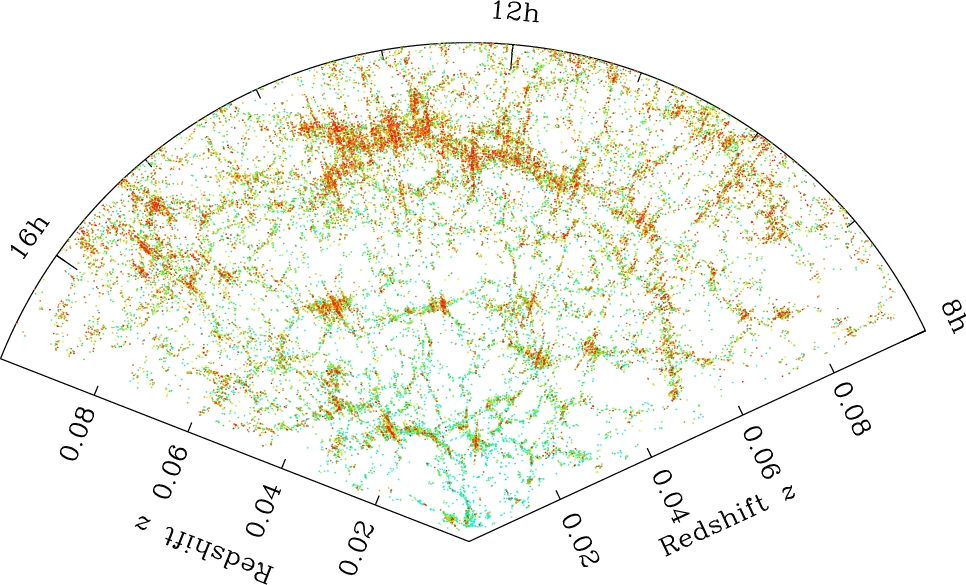
\includegraphics[width=0.5\linewidth]{sdss_voids.jpg}
	\caption{\footnotesize{}Effets de l'allongement des groupes visible sur le relevé du SDSS
	(la couleur sur le graphe traduit celle de la magnitude $B-V$).(\emph{source: http://www.planetastronomy.com)}}
	\label{fig:godfinger}
\end{figure}
La technique habituellement utilisée pour déterminer les groupes est la méthode de la percolation appelée aussi Friends-of-Friends
(FoF) dans l'espace des redshifts qui regroupe toutes les galaxies qui ont des voisines communes (voir la section (\ref{sec:fof})).
Cette technique a également certains désavantages. C'est pourquoi durant le stage, des moyens différents ont été mis en {\oe}uvre
afin de pouvoir aboutir au premier catalogue sur l'ensemble du SDSS-DR7 et qui sera optimal pour gérer les effets de projection et
sélectionner les galaxies dans la sphère virielle. L'idée générale est de remplacer la "simple" méthode de FoF par une sélection de
surdensité dans l'espace projeté et corrigée par un filtrage des vitesses à l'aide de la méthode du maximum de vraisemblance, en
prenant en compte la modélisation des effets de projection faîte par \citet{MBM10} sur des simulations cosmologiques. Ensuite une
fois l'algorithme mis en place, le tester sur des simulations cosmologiques afin d'optimiser quelques paramètres de l'algorithme et
finalement l'appliquer sur le SDSS.

Pour obtenir tous ces résultats, le travail réalisé s'est construit en plusieurs étapes qui vont être décrites dans ce rapport.
\fss{Plan de travail}
Le but final étant de pouvoir réalisé un catalogue des groupes de galaxies et ceci de façon optimale, il est nécessaire de pouvoir
réaliser quelques tests préliminaires du code réalisé pour vérifier qu'il est capable de retrouver des résultats déjà établis.
C'est pourquoi il a fallu tester notre travail sur des simulations cosmologiques. Le choix s'est porté tout d'abord sur la
simulation Millennium II. Une description brève de cette simulation sera faîte afin d'expliquer certains choix effectués durant le
travail. Les données issues de cette simulation ont été traitées et analysées dans le but de simplifier le travail qui devra être
fait par la suite grâce au programme qui a été créé. Une fois les données de la simulation récoltées, un mock catalogue a été créé
pour pouvoir tester par la suite le programme. Un mock catalogue est en quelque sorte une voûte céleste fabriquée de toute pièce à
partir des données d'une simulation cosmologique. Pour être un bon mock catalogue, il faut donc retrouver les propriétés générales
des galaxies enregistrées dans les surveys, tout en gardant également le plus possible les structures aux grandes échelles que
forment les galaxies et les groupes de galaxies. D'une manière générale, on peut dire qu'il faut pouvoir ne pas perdre les
informations contenues dans la simulation, et qu'il ne faut pas en introduire dans le mock catalogue par des biais causés par la
méthode de création de ce mock (qui sera détaillée dans la suite du rapport).

Une fois ce "faux-ciel" créé, le programme de regroupement a été construit en plusieurs étapes lui aussi. Tout d'abord, nous avons
souhaité mettre en place un algorithme similaire à \citet{Yang+07} pour pour pouvoir réaliser des comparaisons entre les
programmes. Ensuite, notre propre algorithme a été développé.

Puis nos algorithmes ont été appliqués sur le mock catalogue qui a été créé, ceci afin d'optimiser les quelques paramètres des
programmes qui ont besoin de l'être et de tester nos programmes.

Mais même ainsi d'autres effets, dus aux limitations mêmes du survey, sont à prendre en compte comme les limites en luminosité et
les effets de bord des surveys (qui tronquent certains amas). Des moyens pour limiter ces effets et les prendre en compte dans le
programme ont été aussi mis en {\oe}uvre pour pouvoir appliquer par la suite notre algorithme sur le SDSS-DR7 en entier, et alors
obtenir les premiers résultats et les exploiter.

Dans la suite du rapport sera donc exposé en détail le travail effectué durant le stage pour aboutir aux résultats qui seront
finalement décrits.
\vspace{1em}
\fs{Création du mock catalogue}
Dans cette section va maintenant être décrit le cheminement pour arriver à créer un mock catalogue qui va permettre de tester les
différents programmes. Il a été construit à partir des données de la simulation Millennium-II et de façon plus précise du catalogue
Guo2010a (\citet{Guo+11}).
\fss{Pourquoi un mock catalogue?}
Les programmes qui ont été réalisés durant le stage doivent pouvoir être testés avant de les lancer directement sur les données du
SDSS DR7. C'est pourquoi le mock catalogue qui a été réalisé est d'une grande aide. En effet certains paramètres des programmes ont
besoin d'être ajustés afin de regrouper au mieux les galaxies, et pour cela il est nécessaire de voir son "comportement" sur des
données dont on connaît la structure à l'avance, c'est-à-dire avoir à disposition un ensemble de données contenant des positions de
galaxies avec d'autres de leurs caractéristiques (comme leur vitesse, leur contenu en masse stellaire, leur magnitude absolue,
etc...) et surtout le groupe auquel elles appartiennent pour pouvoir faire une comparaison avec les résultats donnés par notre
programme. Il s'avère que les simulations cosmologiques permettent d'obtenir de telles informations qui sont ensuite mises à
disposition du "public". C'est ce qui a été fait dans le but de créer le mock catalogue avec la simulation du Millennium-II.
\fss{Obtention des données}
Pour le travail qui est à faire à partir des données du Millennium-II (MSII), le choix qui s'offre à nous est beaucoup trop grand.
Nous n'avons pas intérêt à utiliser l'ensemble des informations qui sont disponibles, c'est pourquoi nous avons dû sélectionner les
données et les analyser afin de se limiter au strict nécessaire en terme de volume de données. Ces choix vont être exposés dans
cette sous-section.
\fsss{La simulation Millennium-II}
La simulation Millennium-II est une simulation à $N$ corps de matière noire dans le cadre d'une cosmologie $\Lambda$CDM (Cold Dark
Matter) \citet{BoylanKolchin+09}. Elle permet d'étudier la formation et l'évolution des structures cosmiques de l'Univers à partir
des résultats obtenus avec la simulation. Celle-ci hérite des caractéristiques de son "ancêtre" la simulation Millennium (MS),
c'est-à-dire qu'elle possède les mêmes paramètres cosmologiques, ainsi que le même nombre de particules de matière noire. Les
différences entre les deux simulations sont que la MSII est réalisée dans une boîte de simulation de côté cinq fois plus petite que
dans le cas de MS avec une résolution spatiale cinq fois meilleure. Il se trouve aussi que la résolution en masse des particules
est 125 fois meilleure elle aussi que dans le cas du MS. Dans les deux cas, des conditions aux limites périodiques sont appliquées
aux bords du cube. Tout ceci tend à nous inciter à l'utilisation des données obtenues à partir de cette simulation. Les paramètres
de la simulation sont résumés dans la table (\ref{tab:param}).
\begin{table}[H]
	\centering
	\begin{tabular}{>{\columncolor{bleu2}}c>{\columncolor{bleu3}}c>{\columncolor{bleu2}}c>{\columncolor{bleu3}}c>{\columncolor{bleu2}}c>{\columncolor{bleu3}}c>{\columncolor{bleu2}}c}
	\hline
		$\Omega_{\rm{tot}}$ & $\Omega_{\rm{m}}$ & $\Omega_{\rm{b}}$ & $\Omega_{\Lambda}$ & $h$ & $\sigma_8$ & $n_s$ \\ \hline
		\num{1.0} & \num{0.25} & \num{0.045} & \num{0.75} & \num{0.73} & \num{0.9} & \num{1} \\ \hline
	\end{tabular}
	\caption{\footnotesize{}Les paramètres cosmologiques utilisés pour la simulation Millennium.}
	\label{tab:param}
\end{table}

Lorsque cette simulation est réalisée, les données (positions, vitesses des particules...) sont régulièrement sauvegardées à
différents "snapshots" ou redshifts, c'est-à-dire à des époques dans la simulation non séparées à des intervalles de temps
réguliers. Pour chacun de ces snapshots on peut appliquer des modèles de formation des galaxies, qui nous seront utiles pour
réaliser le mock. Sur ces snapshots sont appliqués des algorithmes de FoF pour déterminer les halos formés par les particules de
matière noire dans la simulation, puis d'autres algorithmes sont également appliqués afin de raffiner les résultats du FoF et de
détecter les sous-halos parmi les halos trouvés. \`A partir de cela et des caractéristiques de ces halos, on peut appliquer les
modèles de population des galaxies. \`A la suite de ce traitement on a donc des données sur des galaxies avec leurs différentes
propriétés ainsi que leur appartenance vraie à un halo de la simulation, résultant de la manière dont ces galaxies ont été
obtenues.

La simulation de la population galactique que nous avons choisie pour réaliser le mock catalogue est celle du catalogue Guo2010a.
Ce modèle état de l'art permet d'avoir accès à une grande gamme de type de galaxies, la résolution en masse étant assez faible, et
donc d'avoir des galaxies naines dans ce modèle. Ces données sont elles aussi disponibles sur le site du MSII référencées sous
forme de table dans le catalogue Guo2010a, avec les informations sur les halos dans un autre catalogue.

Dans le cadre de notre travail sur le mock, les données ont été filtrées de façon à obtenir que les informations sur les halos et
les galaxies correspondant au dernier snapshot de la simulation à un redshift nul, c'est-à-dire correspondant à notre époque
actuelle, en vue de notre future application du programme sur le SDSS DR7. Mais avant une quelconque utilisation des données à
notre disposition, il est nécessaire de les analyser afin de voir quelles seront les limites de notre mock catalogue et de ne
garder que les informations les plus utiles parmi le large choix offert par cette simulation et le modèle de population galactique
choisi.
\fsss{Analyse des données du catalogue Guo2010a}
La première constatation faîte lors de l'analyse des données du catalogue Guo2010a est le nombre important des informations
disponibles pour chaque galaxie et le nombre de ces galaxies (plus de 13 millions...). Ceci n'est pas sans problème pour la
réalisation du mock catalogue, comme nos moyens informatiques en terme de mémoire sont limités et que le mock catalogue nécessite
un certain nombre de réplication de ces cubes de simulation, et donc un volume de données d'autant plus grand. Il a donc fallu
trouver un moyen de réduire la taille de ces informations tout en évitant les pertes d'informations importantes.
\begin{table}[H]
        \footnotesize
	\centering
	\begin{tabular}{>{\columncolor{bleu2}} c >{\columncolor{bleu3}} c >{\columncolor{bleu2}} c}
	         \hline
	        Nom & Millennium II & Mini MSII \\ \hline
	        $L_{box}$ ($h^{-1}$Mpc) & \num{100} & \num{100} \\ \hline
	        $N_p$ & \num{10077696000} & \num{80621568} \\ \hline
	        $m_p$ ($h^{-1}M_{\odot}$) & \num{6,89e6} & \num{8,61e8} \\ \hline
	        Nombre de galaxies & \num{13191859} & \num{186620} \\
	        du Guo2010a & & \\ \hline
	\end{tabular}
	\caption{\footnotesize{}Les différentes caractéristiques des simulations du Millennium.}
	\label{tab:MScar}
	\normalsize
\end{table}

Une autre simulation du MSII a été réalisée avec un nombre de particules plus faibles et une résolution en masse plus faible pour
les particules de matière noire: il s'agit du mini-MSII. Elle conserve la même taille de côté pour le cube de simulation. Les
différentes propriétés utiles des deux simulations sont résumées dans la table (\ref{tab:MScar}).
\begin{figure}[H]
	\centering
	\includegraphics[width=0.49\linewidth]{massfunc}
	\includegraphics[width=0.49\linewidth]{massfuncII}
	\caption{\footnotesize{}Distribution des masses stellaires pour les deux catalogues Guo2010a obtenus à partir
	du MSII et du mini-MSII.}
	\label{fig:distMste}
\end{figure}

Le fait que les deux simulations aient la même taille de boîte ($L_{box}$) et un nombre de particules de matière noire beaucoup
plus faible dans le cas du mini-MSII est un avantage pour notre mock car le nombre de données à prendre en compte est beaucoup plus
faible et facilement gérable avec nos moyens informatiques. Cependant le fait que la résolution en masse des particules de matière
noire soit plus faible est plus dérangeant car le modèle de population stellaire du catalogue Guo2010a appliqué dans le cas du
mini-MSII donne alors lui aussi une résolution plus faible en terme de masse des galaxies. Celles qui ont une masse faible nous
échappent alors. Ceci est visible lorsque l'on réalise la distribution de masse stellaire des catalogues Guo2010a dans le cas du
MSII et du mini-MSII. Ces distributions sont visibles sur la figure (\ref{fig:distMste}). On voit bien que sur la distribution des
masses dans le cas du MSII on a un "pic" à une masse stellaire presque 100 fois plus faible que dans le mini-MSII. En prenant donc
le mini-MSII à la place du MSII on perd alors l'information dans notre mock sur les galaxies de faible masse.

Maintenant que nous avons fait le choix d'utiliser le catalogue Guo2010a du mini-MSII pour restreindre le volume de données à
traiter pour notre mock catalogue, il faut encore essayer de diminuer le nombre d'informations qui est toujours un peu trop
important. Quand on regarde la distribution des masses stellaires dans le cas du mini-MSII, on voit que les galaxies de masse
stellaire inférieure au pic de la distribution représente une faible part de la population des galaxies. Pourquoi alors ne pas
supprimer de notre mock ces galaxies de faible masse? En regardant la part des galaxies qui ont une masse supérieure à une certaine
masse stellaire, on remarque que cela permettrait de gagner en terme de volume de données tout en ne perdant pas trop
d'informations dans notre mock qui est déjà biaisé par le manque de galaxies de faible masse par le choix de l'utilisation du
mini-MSII. Cette répartition est visible sur la figure (\ref{fig:repMste}).

On voit alors qu'en faisant le choix de ne prendre en compte que les galaxies d'une masse supérieure à \num{e8} $M_{\odot}$ on
réduit fortement le nombre de galaxies à traiter dans le mock tout en ne perdant pas trop d'informations des catalogues car le
choix du mini-MSII nous limite déjà en terme de résolution en masse des galaxies. On peut désormais réaliser le mock catalogue à
partir de ces données avec la méthode qui est décrite dans la partie suivante.
\begin{figure}[H]
	\centering
	\includegraphics[width=0.5\linewidth]{Repfunc}
	\caption{\footnotesize{}Fractions des galaxies du mini-MSII qui ont une masse stellaire supérieure à celle indiquée en
	abscisse.}
	\label{fig:repMste}
\end{figure}
\fss{Réalisation du mock catalogue}
La création du mock catalogue à partir des données de la simulation demande quelques pré-traitements pour éviter certains effets
causés par sa formation à partir de données de simulation et en même temps pour pouvoir conserver les informations qui nous seront
utiles plus tard pour tester notre programme. En effet pour simuler au mieux les données du SDSS certaines des propriétés de notre
mock catalogue doivent correspondre à celles du SDSS comme la magnitude limite par exemple. Ces méthodes vont faire l'objet des
sections suivantes.
\fsss{Informations à conserver pour le mock catalogue}
Avant de voir comment le mock catalogue a été réalisé, il faut connaître les données fournies par le MSII et qui vont nous
permettre de simuler des observations.

Pour tester le programme de regroupement, il nous faut comparer les halos trouvés par notre algorithme avec ceux de la simulation
du MSII. Deux catalogues sont disponibles à partir de cette simulation: un catalogue contenant des informations sur les halos de
matière noire comme leurs positions, leurs vitesses, etc..., ainsi qu'un catalogue sur les galaxies qui peuplent ces halos avec de
nombreuses caractéristiques. Le nombre de données étant assez élevé dans les deux catalogues, une simple comparaison une à une des
données entre les deux pour associer à chaque galaxie les caractéristiques du halo auquel elle appartient dans la simulation
donnerait un temps de calcul prohibitif. On a donc mis en place un algorithme pour réaliser un matching plus rapide pour faire
cette correspondance (non détaillé).%\com{Peut être mettre le code ou algo en annexe}

Nous avons désormais les données utiles pour la réalisation du mock catalogue, car nous avons la correspondance entre les données
des halos et des galaxies.
\fsss{Méthodes de création du mock catalogue\label{sec:galcarac}}
Pour notre mock, nous avons besoin de données pouvant simuler des observations réalisées sur un intervalle de redshift compatible
avec celui du relevé qu'on simule, c'est à dire dans notre cas le SDSS. On doit alors atteindre une profondeur en redshift de près
de $z=\num{0.3}$. Cependant on l'a vu la taille de la boîte de la simulation du MSII est de \num{100} $h^{-1}$Mpc ce qui équivaut à
une profondeur en redshift de $z\sim\num{0.03}$, bien inférieure à la valeur nécessaire pour simuler le SDSS. C'est pourquoi pour
créer le mock catalogue nous avons répliquer la boîte de simulation pour atteindre la profondeur souhaitée.

Mais pour cela il faut appliquer quelques transformations à cette boîte afin de limiter certains biais qui pourraient être
introduits par cette réplication.
\fssss{Réplication du cube de simulation}
La façon de procéder pour aboutir à notre mock catalogue est assez simple sur le principe: on va juxtaposer des cubes de la
simulation du MSII (comme celui de la figure (\ref{fig:cube})) les uns aux autres afin d'atteindre la profondeur
\begin{figure}[htb]
	\centering
%	\includegraphics[width=0.5\linewidth]{cubemock}
	\caption{\footnotesize{}Le cube du mini-MSII avec les galaxies du Guo2010a. La couleur d'une galaxie dépend du halo auquel
	elle est associé (à chaque couleur correspond un halo).}
	\label{fig:cube}
\end{figure}
souhaitée pour correspondre aux données du SDSS. En se contentant de faire ce travail, en translatant les positions des galaxies
pour chaque cube que l'on accole aux précédents, on introduit des biais dans le mock. En effet si on superpose ainsi les cubes les
uns aux autres, on va répliquer une même image du ciel mais à différentes distances. Du coup, si on se place à un endroit dans le
cube de notre mock et que l'on observe dans une direction du cube (comme dans le cas d'un télescope observant une portion du ciel),
on remarque un effet de perspective dans le ciel causé par cette réplication comme dans la figure (\ref{fig:perspective}).
\begin{figure}[htb]
        \centering
	\includegraphics[width=0.5\linewidth]{perspective.png}
	\caption{\footnotesize{}Effet de perspective dans un mock réalisé avec une simple superposition de cubes
	(projection angulaire), les ascensions droites (RA) et les déclinaisons (DEC) sont arbitraires et
	représentent seulement des directions orthogonales dans la "fausse voûte céleste", d'après \citet{Blaizot+05}.}
	\label{fig:perspective}
\end{figure}

Pour pallier à ce problème, une technique consiste à faire subir des transformations supplémentaires à chaque cube de manière
aléatoire pour éviter les répliques parfaitement identiques comme décrit dans \citet{Blaizot+05}. Pour cela on va effectuer trois
transformations différentes sur les coordonnées du cube, en plus des simples translations suivant les axes ($X,Y,Z$), pour pouvoir
accoler les cubes les uns aux autres.

\noindent{\eeent{1}} La première transformation est une rotation d'un angle multiple du demi-entier de $\pi$ autour de chacun des
trois axes du cube, chaque angle étant éventuellement différent. Le choix du multiple pour l'angle de rotation doit se faire
aléatoirement afin de ne pas introduire de nouveaux effets de perspective par ces rotations. On choisit un angle aléatoire multiple
demi-entier de $\pi$ et non pas un angle compris dans l'intervalle continu $[0,2\pi]$ pour ne pas perdre des informations sur les
halos dans le cube de simulation. En choisissant un angle multiple de $\frac{\pi}{2}$, on permet à chaque galaxie de se retrouver à
nouveau dans le "même" cube de simulation qu'auparavant mais avec des coordonnées différentes. Nous n'avons pas alors à récupérer
des galaxies qui sortiraient de cette boîte pour les y remettre à l'aide de conditions périodiques aux limites qui
"déstructureraient" complètement notre cube, et les informations sur l'appartenance d'une galaxie à un certain halo deviendraient
totalement inutilisables. On peut voir ceci sur la figure (\ref{fig:cube2}).
\begin{figure}[htb]
	\centering
	\includegraphics[width=0.4\linewidth]{cube.pdf}
	\caption{\footnotesize{}Illustration de l'effet d'une rotation quelconque du cube. On voit que l'application des conditions
	périodiques sur le cube bleu inscriraient des zones vides dans le cube vert ou des zones de sur-densités. On perdrait alors
	des informations du MSII.}
	\label{fig:cube2}
\end{figure}

\noindent{\eeent{2}} La deuxième transformation est une translation d'une longueur comprise dans l'intervalle continu de
$[0,L_{box}]$. On pousse les galaxies du cube suivant une direction sur une longueur choisit aléatoirement dans l'intervalle
précédent, et celles qui en sortent sont ramenées dans le cube de l'autre côté en appliquant des conditions aux limites
périodiques.

\noindent{\eeent{3}} La troisième et dernière transformation est une inversion choisit aléatoirement suivant l'un des trois axes du
cube. Il peut aussi n'y avoir aucune inversion appliquée à l'ensemble des trois axes.

Avant de pouvoir réaliser ces transformations pour faciliter la suite des calculs, on décale l'origine de la boîte de simulation du
MSII qui est située sur un coin pour la placer au centre. Ensuite on peut appliquer les transformations aléatoires sur les
coordonnées des galaxies du cube et les translations sur les coordonnées pour placer chacun des cubes dans notre mock, tout ceci
pouvant être résumé de la façon suivante:
\begin{eq}
        \textbf{X'}=\mathcal{I}_{XYZ}\mathcal{R}_{X}(\theta_{X})\mathcal{R}_{Y}(\theta_{Y})\mathcal{R}_{Z}(\theta_{Z})\textbf{X}+\textbf{T}
\end{eq}
où $\textbf{X'}$ représente les coordonnées $\textbf{X}$ suivant les trois axes du cube d'une galaxie une fois transformées,
$\mathcal{R}_i$ la rotation suivant l'axe $i$ d'un angle multiple de $\frac{\pi}{2}$ aléatoire $\theta_i$, $\mathcal{I}$
l'inversion suivant un des trois axes (qui peut ne pas être réalisé) et $\textbf{T}$ la translation qui va permettre de placer le
cube dans la grande boîte du mock catalogue.

Une fois que ces transformations ont été réalisées sur le cube, celui-ci est juxtaposé aux autres cubes déjà placés en effectuant
une translation des coordonnées des galaxies suivant les axes du cube de la longueur nécessaire pour placer correctement la boîte
de la simulation parmi les autres. On obtient de cette façon un cube plus gros comme sur la figure
(\ref{fig:mock}). De cette façon, les effets de perspective ne peuvent plus être visibles sur notre fausse voûte
céleste comme on peut le voir sur la figure (\ref{fig:hom}) dans le cas d'un mock où cette méthode a été testée.
\begin{figure}[htb]
	\centering
	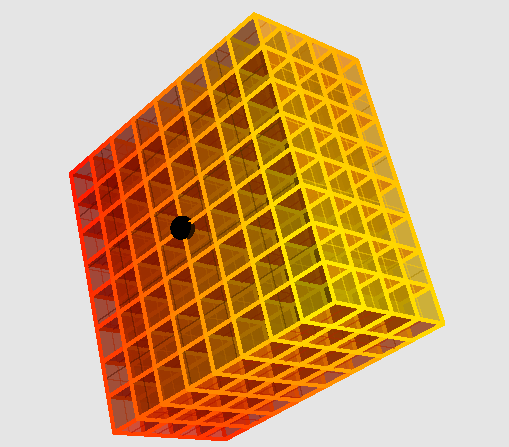
\includegraphics[width=0.4\linewidth]{mock}
	\caption{\footnotesize{}Une image du \emph{gros} cube du mock réalisé en juxtaposant les différents cubes engendrés par transformation du cube initial.}
	\label{fig:mock}
\end{figure}
\begin{figure}[htb]
	\centering
	\includegraphics[width=0.5\linewidth]{random.png}
	\caption{\footnotesize{}Cas d'un mock réalisé avec la méthode décrite dans l'article sur MoMaF: le faux-ciel semble
	homogène et les effets de perspective causés par la réplication du cube ne sont plus visibles, d'après \citet{Blaizot+05}.}
	\label{fig:hom}
\end{figure}
Le mock catalogue ainsi crée et visible sur l'image ne présente plus d'effets de perspective causés par la réplication d'un même
cube un certain nombre de fois. Le résultat est tout à fait semblable à ce que l'on pourrait obtenir en prenant directement une
simulation réalisée dans une boîte de taille équivalente à la profondeur en redshift que l'on souhaite avoir pour notre mock
catalogue.

Avec ce simple travail on ne peut pas dire que le mock créé est comparable au SDSS, c'est pourquoi il est nécessaire d'ajouter des
caractéristiques et des biais qui vont permettre d'obtenir des données au comportement presque identique à celles du SDSS.
\fssss{Ajout de caractéristiques aux données}
Une caractéristique importante du SDSS est le fait que l'on est sensible seulement à des galaxies qui ont une magnitude inférieure
à une magnitude limite. Pour ajouter cet effet dans notre mock catalogue, il nous faut obtenir les magnitudes apparentes des
galaxies de notre mock. Or les magnitudes apparentes sont des caractéristiques qui dépendent de l'observateur, ce qui nous amène à
définir la position de cet observateur dans le cube de notre mock catalogue. L'origine des coordonnées de ce cube est située dans
un de ses coins et semble être un bon choix pour la position de l'observateur car cela nous permettra de déterminer des coordonnées
d'ascension droite et de déclinaison très facilement à partir des coordonnées cartésiennes des galaxies.

Dans notre mock catalogue nous avons à disposition les magnitudes absolues de chacune des galaxies qui découlent du modèle de
population galactique appliqué sur la simulation du MSII. On souhaite obtenir à partir de cela les magnitudes apparentes vues
depuis l'observateur (situé à l'origine de notre mock). Les effets qui contribuent à donner une certaine magnitude apparente $m$
d'une galaxie d'une magnitude absolue $M$ sont la distance à l'observateur ainsi que le décalage spectral du flux de la galaxie
causé par l'expansion. L'extinction provoquée par les diverses poussières interstellaires sur la ligne de visée à l'observateur ne
sont pas prises en compte dans notre mock étant donné le manque d'information pour appliquer ce type de correction dans les données
de la simulation. Tout ceci peut être résumé par l'expression suivante:
\begin{eq}\label{eq:corrobs}
        m_X=M_X+5\log_{10}{d_{\rm{lum}}(pc)}-5+K(z,m_X-m_{X'})
\end{eq}
où $X$ représente une des bandes de longueurs d'onde dans lesquelles sont exprimées les magnitudes absolues du MSII qui
correspondent à celles du SDSS ($u,g,r,i,z$), $K$ est la correction appliquée pour tenir compte du décalage spectral du flux de la
galaxie (appelée "correction-K" dans la suite) et $d_{\rm{lum}}$ la distance lumineuse de la galaxie basée sur la conservation de
la loi de diminution de la luminosité en fonction de la distance comme définie dans un Univers euclidien.

Le calcul de $K$ est basé sur les résultats de \citet{CMAZ10} qui permet de calculer cette correction à partir d'une expression
sous la forme d'un polynôme du redshift et de la couleur pour certaines bandes du SDSS. Les coefficients du polynôme dans les
différents cas proposés sont tabulés et cette correction a pu être programmée avec ces coefficients. On remarque aussi un autre
problème pour calculer la magnitude apparente avec l'équation (\ref{eq:corrobs}): pour la correction-K il est nécessaire de
connaître la magnitude apparente déjà dans une autre bande pour calculer la magnitude apparente dans une bande. La méthode qui a
été utilisée tout d'abord est le calcul de cette magnitude de façon itérative. Dans un premier temps, on réalise le calcul à l'aide
des magnitudes absolues dans la correction-K:
\begin{eq}
        m_X^{(1)}=M_X+5\log_{10}{d_{\rm{lum}}(pc)}-5+K(z,M_X-M_{X'})
\end{eq}
puis pour les itérations suivantes on injecte dans $K$ les valeurs des magnitudes apparentes calculées précédemment, et tant que la
différence des valeurs des magnitudes entre deux itérations successives ${\Delta}m=|m^{(i)}-m^{(i+1)}|$ est supérieure à
\num{0,01}:
\begin{eq}
        m_X^{(i+1)}=M_X+5\log_{10}{d_{\rm{lum}}(pc)}-5+K(z,m_X^{(i)}-m_{X'}^{(i)})
\end{eq}
Le redshift $z$ de la galaxie du mock est estimé à partir de la distance comobile $D[h^{-1} Mpc]$ qui est donnée par les positions
comobiles de la galaxie dans le MSII. Pour le calcul de la distance lumineuse, on utlise une approximation analytique donnée par
\citet{WU10} dont la précision est suffisante aux redshifts où on travaille. La distance comobile étant égale à la distance de
\emph{mouvement propre} dans la cas d'un Univers plat et connaissant la relation entre distance de mouvement propre et la distance
de luminosité, on peut alors en inversant la relation entre distance lumineuse et redshift, déterminer ce dernier à partir de la
distance comobile. Pour cela, on détermine pour différents échantillons de $z$ les valeurs de la distance comobile sur l'intervalle
de $z$ qui nous intéresse, puis en s'aidant d'une interpolation à splines cubiques, on peut connaître le $z$ correspondant à une
distance comobile donnée.

Pour avoir une autre vérification de nos résultats sur les magnitudes apparentes (car elles ne convergent pas toutes vers une
valeur physique par la méthode de l'itération), on a tenté de résoudre le système cubique formé par les magnitudes apparentes avec
l'approximation donnée par \citet{CMAZ10}. Quand on regarde l'expression de la K-correction analytique, elle s'exprime comme:
\begin{eq}
        K(z,m_{X}-{m}_{X'})=\sum_{i=0}^{N_i}\sum_{j=0}^{N_j}{a_{ij}}{z^i}{(m_X-{m}_{X'})^j}
\end{eq}
avec $N_i$ et $N_j$ qui représentent les ordres des polynômes utilisés pour l'approximation et $a_{ij}$ les coefficients d'une
matrice $N_i\times{N_j}$. Si on connaît le redshift, on remarque que déterminer les magnitudes apparentes revient à résoudre un
système polynomial (et non linéaire) d'ordre $N_j$. Dans ce cas, $N_j=3$ donc le système est d'ordre 3. En utilisant un
sous-programme de résolution de systèmes non linéaires de \citet{NumericalRecipes}, on remonte ainsi à chacune des magnitudes
apparentes voulues. En faisant la comparaison avec la méthode par itération décrite précédemment, les résultats obtenus sont
sensiblement identiques, les différences étant visibles à l'ordre \num{e-3}. Malheureusement, de temps à autre, le calcul des
magnitudes apparentes selon les deux méthodes peut ne pas aboutir à une solution physique (divergence vers des valeurs très grandes
ou très négatives). On a alors choisi d'adopter une solution simple. La méthode est la suivante: on commence à chercher une
solution numérique au système d'équation réalisée uniquement par les magnitudes apparentes en bande $r$ et $g$ pour limiter les
problèmes de non-convergence plus fréquent quand on cherche à déterminer les solutions pour les cinq bandes $u,g,r,i,z$. Si aucune
solution n'a été trouvée ou si la solution n'est pas réaliste, on tente à nouveau de déterminer les magnitudes apparentes par des
itérations. Si pour les mêmes raisons que précédemment on ne trouve pas de \emph{bonnes} solutions, on se contente de corriger la
magnitude absolue du module de distance ($m_X=M_X+5\logg{d_{\rm{lum}}}(pc)-5$), et la galaxie se voit affecter un \emph{flag} dans
le mock catalogue. D'après les flags du mock catalogue, la combinaison des deux méthodes, l'une prenant le relais de l'autre quand
elle a échoué, empêche d'aboutir à des galaxies non K-corrigée au final car aucun flag ne signale la présence d'une galaxie
seulement corrigée du module de distance.

On peut alors de cette manière déterminer les magnitudes apparentes de chaque galaxie de notre mock. Pour pouvoir être réaliste, on
rajoute alors un filtrage en magnitude dans le mock catalogue, en ne gardant que les galaxies qui ont une magnitude apparente
$m_{r}<\num{17,77}$ dans la bande $r$ pour correspondre à la limite en flux du SDSS.

Le mock catalogue doit permettre de simuler des observations sur une fausse voûte céleste, il faut donc attribuer des coordonnées
équatoriales à chacune des galaxies. Pour cela on va utiliser les propriétés du cube de notre mock pour calculer ces coordonnées. On
va supposer que le plan ($X,Y$) du cube est le plan équatorial et l'axe $Z$ dans le sens positif donne l'axe du pôle céleste (en
direction du pôle Nord). Les ascensions droites sont comptées positivement dans le sens indirect pour correspondre aux "véritables"
coordonnées. L'origine est toujours l'observateur. Pour le calcul on va partir des coordonnées sphériques pour déterminer les
expressions des ascensions droites $\alpha$ et des déclinaisons $\delta$. Les coordonnées cartésiennes ($X,Y,Z$) s'écrivent à partir
des sphériques ($r,\phi,\theta$):
\begin{eqnarray}
        X&=&r\cos\phi\sin\theta \nonumber\\
        Y&=&r\sin\phi\sin\theta \nonumber\\
        Z&=&r\cos\theta \nonumber\\
\end{eqnarray}
Pour les ($\alpha,\delta$), on a $\phi=2\pi-\alpha$ et $\theta=\frac{\pi}{2}-\delta$. On peut donc réécrire:
\begin{eqnarray}
        X&=&r\cos\alpha\cos\delta \nonumber\\
        Y&=&-r\sin\alpha\cos\delta \nonumber\\
        Z&=&r\sin\delta \nonumber\\
\end{eqnarray}
On détermine alors les coordonnées en appliquant une dernière transformation à $\alpha$ pour ramener les valeurs dans l'intervalle
[$0,2\pi$]:
\begin{eq}
        \alpha=\left\{ \begin{array}{lcr}
                         -\mbox{arctan2}(Y,X)+2\pi & \mbox{si} & Y>0 \\
                         -\mbox{arctan2}(Y,X) & \mbox{sinon} & \\
                        \end{array}\right.\nonumber
\end{eq}
\begin{eq}
        \delta=\mbox{signe}(Z)\arccos\left(\frac{\sqrt{X^2+Y^2}}{\sqrt{X^2+Y^2+Z^2}}\right)
\end{eq}

Afin de réduire la taille des données et le temps de calcul de leur traitement, le calcul des magnitudes apparentes ainsi que le
filtrage sont réalisés pendant la génération de chaque sous-cube du mock catalogue.

Le redshift que l'on détermine ici pour le calcul de la magnitude apparente est un redshift \emph{vrai} c'est-à-dire le redshift
causé seulement par l'expansion de l'Univers et qui traduit la distance à laquelle se trouve la galaxie. Cependant comme on l'a vu
dans la section (\ref{sec:elong}), il y a des effets d'élongation des groupes dans l'espace des redshifts causés par l'accumulation
de la vitesse du \textit{Hubble flow} (expansion) et de la vitesse particulière de la galaxie. On doit donc déterminer nous aussi
un redshift "observationnel" pour notre mock catalogue afin de simuler correctement le SDSS. Pour cela on doit déterminer la
vitesse particulière $v_{\rm{pec}}$ de chaque galaxie. Les composantes suivant les trois axes du cube de simulation sont données
dans le Guo2010a. Il suffit alors de calculer la vitesse projetée sur la ligne de visée de l'observateur pour avoir le redshift.
Celui-ci est calculé de la façon suivante:
\begin{eq}
        1+z=\sqrt{\frac{1+\frac{v}{c}}{1-\frac{v}{c}}}
\end{eq}
avec $v$ la vitesse algébrique suivant la ligne de visée donc $v=v_{\rm{pec}}+v_{\rm{flow}}$ où $v_{\rm{pec}}$ la vitesse
particulière projetée de la galaxie et $v_{\rm{flow}}=\num{100}{\times}D[h^{-1}Mpc]$ la vitesse causée par l'expansion avec $D$ la distance
comobile de la galaxie accessible \emph{via} le Guo2010a.

On rappelle aussi que l'intérêt de créer un mock catalogue est de posséder l'information déjà connue à l'avance de l'appartenance
d'une galaxie à un halo. Après avoir réaliser le \emph{matching} entre les galaxies et le halo, on a déterminé la zone où se trouve
la galaxie afin de réaliser nos futures comparaisons. Il suffit de calculer pour cela $r_{\rm{3D}}/r_{\rm{vir}}$ où $r_{\rm{3D}}$
est la distance au centre du halo de la galaxie et $r_{\rm{vir}}$ le rayon de viriel estimé à partir de la masse de la masse du
halo. On en profite pour donner la relation entre la masse du halo et le rayon de viriel et poser une définition. Si on note
$M_{\rm{vir}}$ la masse du halo, alors:
\begin{eq}
        M_{\rm{vir}}=\frac{\Delta}{2}\frac{H_0^2{r_{\rm{vir}}}^3}{G}
\end{eq}
avec $\Delta$ la valeur de la sur-densité. On définit alors $r_{\Delta}$ le rayon de viriel à la valeur de la sur-densité $\Delta$
(par exemple \num{180}). C'est le rayon du halo où la densité est $\Delta$ fois supérieure à la densité crtique $\rho_c$ avec:
\begin{eq}
        \rho_c=\frac{3{H_0^2}}{8\pi{G}}
\end{eq}

On dispose alors d'un mock catalogue contenant les données qui sont résumées dans la table (\ref{tab:donnees}).
\begin{table}[htb]
        \footnotesize
	\centering
	%\rowcolors{2}{bleu2}{bleu3}
	\begin{tabular}{| >{\columncolor{bleu2}} c| >{\columncolor{bleu3}} c|}
	        \hline
		\rowcolor{viol}Numéro & Description \\
		\hline\hline
		1 & Numéro du cube \\ \hline
		2 & Identité dans le cube \\ \hline
		3 & Identité du halo \\ \hline
		4 & Ascension droite \\ \hline
		5 & Déclinaison \\ \hline
		6 & Position comobile $X$ \\ \hline
		7 & Position comobile $Y$ \\ \hline
		8 & Position comobile $Z$ \\ \hline
		9 & Vitesse suivant $X$ \\ \hline
		10 & Vitesse suivant $Y$ \\ \hline
		11 & Vitesse suivant $Z$ \\ \hline
		12 & $m_g$ \\ \hline
		13 & $m_r$ \\ \hline
		14 & $M_g$ \\ \hline
		15 & $M_r$ \\ \hline
		16 & Distance comobile \\ \hline
		17 & Redshift vrai $z$ de la galaxie \\ \hline
		18 & Redshift observé $z$ de la galaxie \\ \hline
		19 & $r_{\rm{3D}}/r_{\rm{vir}}$ \\ \hline
		... & Autres informations du Guo2010a \\
		\hline
	\end{tabular}
	\caption{\footnotesize{}Résumé des données fournies par notre mock catalogue pour chaque galaxie.}
	\label{tab:donnees}
	\normalsize
\end{table}
\fsss{Vérification simple}
Une vérification simple, pour voir si notre mock catalogue est cohérent avec notre idée de simuler le SDSS, doit être réalisée.
D'une façon simple, on s'attend à avoir un rougissement des galaxies quand elles sont éloignées de l'observateur (voir
\citet{Blaizot+05}), et à cause de la limite en flux que l'on impose au mock catalogue on doit avoir moins de galaxies dans notre
mock quand on s'éloigne de l'observateur. C'est ce qui semble être visible sur le mock catalogue quand on regarde la figure
(\ref{fig:mocktr}). On observe effectivement moins de galaxies quand le redshift devient plus grand, et un rougissement ($(g-r)$ de
plus en plus petit traduit par une couleur qui passe du vert au rouge sur la figure (\ref{fig:mocktr})) vers les grands redshifts.
L'autre effet de l'élongation des groupes est lui aussi bien modélisé car on voit des \emph{doigts} pointés vers l'observateur à
l'origine.

\fss{Limitations du mock catalogue}
La raison pour laquelle on a créé ce mock catalogue est que l'on souhaite obtenir un faux catalogue possédant au mieux les
propriétés du SDSS, tout en ayant à notre disposition les informations d'appartenance des galaxies à un halo de façon certaine, ce
qui est fourni par les données du MSII. Pour avoir une profondeur en redshift suffisante, il nous a fallu répliquer la boîte de la
simulation du MSII. Sur cette boîte des conditions aux limites périodiques sont appliquées afin de déterminer les halos de
particules de matière noire, donc certaines galaxies sur un des bords de la boîte peuvent être regroupées avec des galaxies situées
sur une autre face du cube. On voit alors qu'en juxtaposant ces boîtes pour créer notre mock, si on cherche à y retrouver des
groupes qui sont aux bords des cubes juxtaposés, on fera un lien entre des galaxies de cubes différents car nos transformations
aléatoires auront crées ces structures, mais les informations d'appartenance ou non au halo données par le MSII seront faussées
dans ce cas par la faute des conditions aux limites. Il faudra alors tenir compte de cet effet quand on appliquera les algorithmes
de groupe sur ce mock, et peut être essayer de le quantifier pour corriger nos résultats.
\begin{figure}[htb]
	\centering
%	\includegraphics[width=0.5\linewidth]{tranche.pdf}
	\caption{\footnotesize{}Une \emph{tranche} du mock catalogue sélectionnée avec $\delta$>\num{1.0} et $\delta$<\num{1.3}
	$radians$ ainsi que $z<0.25$ pour les galaxies. On observe bien une évolution de la couleur des couleurs des galaxies
	($g-r$) avec le redshift, celles-ci devenant plus rouges quand on s'éloigne de l'observateur. Le mock étant vu sur un coin
	par l'observateur, les ascensions droites sont comprises entre $3\pi/2$ et $2\pi$ ce qui forme un angle droit sur l'image.
	On remarque aussi les effets d'élongation qui ont bien été modélisés, le redshift étant celui observé sur la figure.}
	\label{fig:mocktr}
\end{figure}

Il a fallu ensuite réaliser l'algorithme de \citet{Yang+07} pour tester un autre algorithme en comparaison de celui que l'on va
réaliser, et voir ainsi les différences entre les programmes appliqués sur le mock catalogue et sur le SDSS-DR7.
\fs{L'algorithme de Yang \textit{et al.}}
Cet algorithme va tout d'abord être décrit puis le travail réalisé pour l'implémenter également et finalement les résultats qui
auront été obtenus seront discutés pour vérifier le bon fonctionnement de ce programme.
\fss{Description\label{sec:et4}}
L'algorithme de \citet{Yang+07} permet de déterminer les groupes de galaxies et d'obtenir certaines caractéristiques de ces groupes
comme la masse stellaire par exemple. Le travail décrit dans \citet{Yang+07} se base sur les données du SDSS-DR4 mais le principe
général peut être également appliqué sur le SDSS-DR7. Les données utilisées sont les redshifts des galaxies lorsqu'ils étaient sûrs
ainsi que les magnitudes absolues corrigées de l'extinction et de la correction-K d'une façon qui ne sera pas décrite ici mais que
l'on peut voir dans \citet{Yang+07}. Dans une première approximation, les masses stellaires sont déterminées à partir des
magnitudes absolues selon l'expression suivante:
\begin{eqnarray}\label{eq:mstel}
        \logg\left(\frac{M_*}{{h^{-2}}{M_{\odot}}}\right)&=&\num{-0,306}+\num{1,097}(g-r)-\num{0,1}\nonumber\\
                                                         & &-\num{0,4}(M_r-5\logg{h}-M_{r,\odot})\nonumber\\
\end{eqnarray}
avec $M_*$ la masse stellaire de la galaxie, $(g-r)$ la couleur corrigée de la galaxie, $M_r$ la magnitude absolue K-corrigée
en bande $r$ et $M_{r,\odot}=\num{4,64}$ la magnitude absolue du Soleil en bande $r$.

La détermination des groupes avec cet algorithme s'organise en 5 étapes principales qui vont faire l'objet de ce qui suit.

\noindent{\ent{1}} Tout d'abord trouver le centre potentiel des groupes. Pour cela, un algorithme de FoF est appliqué sur les
galaxies pour déterminer des groupes potentiels, qui représenteraient plutôt la partie centrale des groupes "réels" car le
paramètre qui définit le lien ou non entre les galaxies est choisi petit et différent selon la direction de la ligne de visée
(espace de redshift) et selon la direction transverse. Il est plus grand dans le cas de la ligne de visée pour prendre les galaxies
qui seraient éloignées du groupe par l'effet de l'élongation décrit dans la section (\ref{sec:elong}). Ensuite le "barycentre
lumineux" (voir la section (\ref{sec:annbar})) est calculé pour chaque groupe potentiel et est défini comme le centre du groupe.
Toutes les galaxies non liées à un groupe sont gardées et traitées comme des groupes potentiels elles aussi.

\noindent{\ent{2}} Il faut maintenant déterminer la luminosité caractéristique de ces groupes potentiels. On ne garde dans ce cas
là que les galaxies ayant une magnitude absolue en bande $r$ telle que:
\begin{eq}\label{eq:mchar}
        M_r\leq\num{-19,5}
\end{eq}
Avec ce choix de magnitude, tous les groupes avec un redshift $z\leq\num{0,09}$ et avec des galaxies qui répondent au critère de
(\ref{eq:mchar}) sont visibles: on dit que le groupe est complet. Dans ce cas la luminosité caractéristique $L_{\num{19,5}}$ ce
calcul comme:
\begin{eq}
        L_{\num{19,5}}=\sum_i{\frac{L_i}{\mathcal{C}_i}}
\end{eq}
où $\mathcal{C}_i$ est la complétude du survey à la position de la galaxie $i$, et $i$ court sur les galaxies du groupe qui
vérifient (\ref{eq:mchar}). Pour notre mock catalogue $\mathcal{C}_i$ vaut 1 car toutes les galaxies sont comptées. Si le groupe
n'est pas complet (i.e. z>\num{0.09}) alors la luminosité est:
\begin{eq}
        L_{\num{19,5}}=\frac{1}{f(L_{\num{19,5}},L_{lim})}\sum_i{\frac{L_i}{\mathcal{C}_i}}
\end{eq}
avec $L_{lim}$ la luminosité limite au redshift du groupe, et $f(L_{\num{19,5}},L_{lim})$ un facteur de correction pour prendre en
compte les galaxies manquantes par le flux limite du SDSS, qui sera détaillé plus tard.

On calcule aussi les masses stellaires des groupes selon le même principe que pour les luminosités en sommant les masses stellaires
des galaxies du groupe, et en corrigeant de la même façon quand le groupe n'est pas complet en utilisant un facteur de correction
$g(L_{\num{19,5}},L_{lim})$ qui est calculé selon la même méthode que pour les luminosités mais pas pour la première itération. Les
masses stellaires utilisées sont celles des galaxies qui répondent au critère de luminosité définit ci-dessus dans le groupe.

\noindent{\ent{3}} On détermine maintenant les différentes caractéristiques de ces groupes. La masse du halo $M_h$ est d'abord
estimée à partir de la relation masse-luminosité suivante:
\begin{eq}
        \frac{M_h}{L_{\num{19,5}}}=\num{500}h\frac{M_{\odot}}{L_{\odot}}
\end{eq}
Pour les itérations suivantes, on utilisera la relation $\frac{M_h}{L_{\num{19,5}}}-L_{\num{19,5}}$ que l'on déterminera et qui
sera détaillée dans la suite.

\noindent{}Le halo de matière noire est défini comme ayant une surdensité de 180 donc son rayon est calculé comme:
\begin{eq}
        r_{180}=\num{1,26}{h^{-1}}\mbox{Mpc}{\left(\frac{M_h}{\num{e14}{h^{-1}}M_{\odot}}\right)}^{1/3}(1+z_{group})^{-1}
\end{eq}
où $z_{group}$ est le redshift du centre du groupe.

\noindent{}La dispersion de vitesse sur la ligne de visée est calculée comme:
\begin{eq}
        \sigma=\unit{\num{397,9}}{\kilo\meter.\reciprocal\second}{\left(\frac{M_h}{\num{e14}{h^{-1}}M_{\odot}}\right)}^{\num{0,3214}}
\end{eq}

\noindent{}\ent{4} Mise à jour des groupes avec les informations du halo déterminées précédemment. Le nombre de contraste de
densité aux alentours du centre du halo (confondu avec celui du groupe) peut s'écrire:
\begin{eq}
        P_M(R,\Delta{z})=\frac{H_0}{c}\frac{\Sigma(R)}{\bar{\rho}}p(\Delta{z})
\end{eq}
avec $\Delta{z}=z-z_{group}$ où $z$ est le redshift de la galaxie en question, $\bar{\rho}$ la densité moyenne de l'Univers et
$\Sigma(R)={2}{r_s}{\bar{\delta}}{\bar{\rho}}{f(R/r_s)}$ la densité surfacique projetée pour un modèle de halo NFW
(Navarro-Frenk-White, \citet{NFW97}), avec $r_s$ le rayon d'échelle. La fonction $f$ s'écrit:
\begin{eq}
        f(x)= \left\{ \begin{array}{lr}
                                \frac{1}{x^2-1}\left\{1-\frac{\ln{\left[(1+\sqrt{1-x^2})/x\right]}}{\sqrt{1-x^2}}\right\}, & x<1 \\
                                1/3, & x=1 \\
                                \frac{1}{x^2-1}\left({1-\frac{\arctan{\sqrt{x^2-1}}}{\sqrt{x^2-1}}}\right), & x>1 \\
                      \end{array}\right.
\end{eq}
et avec aussi:
\begin{eq}
        \bar{\delta}=\frac{180}{3}\frac{c_{180}^3}{\ln(1+c_{180})-c_{180}/(1+c_{180})}
\end{eq}
où $c_{180}=r_{180}/r_s$. La fonction $p(\Delta{z})d\Delta{z}$ décrit la distribution en redshift et est supposée avoir une forme
gaussienne:
\begin{eq}
        p(\Delta{z})=\frac{1}{\sqrt{2\pi}}\frac{c}{\sigma(1+z_{group})}\exp\left[\frac{-(c\Delta{z})^2}{2\sigma^2(1+z_{group})^2}\right]
\end{eq}

\noindent{}La façon de procéder est la suivante: pour chaque galaxie on boucle sur les groupes et on fait le calcul de $R$ et de
$z$, où $R$ est la distance projetée au centre du groupe au redshift du groupe. Si $P_M(R,\Delta{z})\geq{B}$ avec $B=\num{10}$
choisit en fonction de précédents résultats, alors la galaxie appartient à ce groupe. Si elle peut être associée à plus d'un groupe
par ce critère, alors on l'associe au groupe pour lequel $P_M(R,\Delta{z})$ est le plus grand.

\noindent{}\ent{5} Finalement en utilisant les nouveaux membres de groupe de l'étape précédente, on calcule à nouveau les centres
de groupes puis on retourne à l'étape \eent{2}. Ceci se déroule tant qu'il y a des changements dans les groupes. \`A partir de ces
groupes, on détermine la fonction de correction des luminosités $f(L_{\num{19,5}},L_{lim})$ ainsi que la relation masse-luminosité
et on retourne à l'étape \eent{1}. Cette boucle s'achève une fois que la relation masse-luminosité a convergé.

Bien que les différents choix initiaux pour les différentes fonctions de correction comme $f(L_{\num{19,5}},L_{lim})$ ou la
relation masse-luminosité soient grossiers, le fait de réaliser le calcul de manière itérative permet de gagner en précision car
ces fonctions sont ensuite consistantes avec les données et les informations des groupes eux-mêmes. L'ensemble de ces étapes est résumé
sur la figure (\ref{fig:diag}).

\begin{figure}[htb]
	\centering
	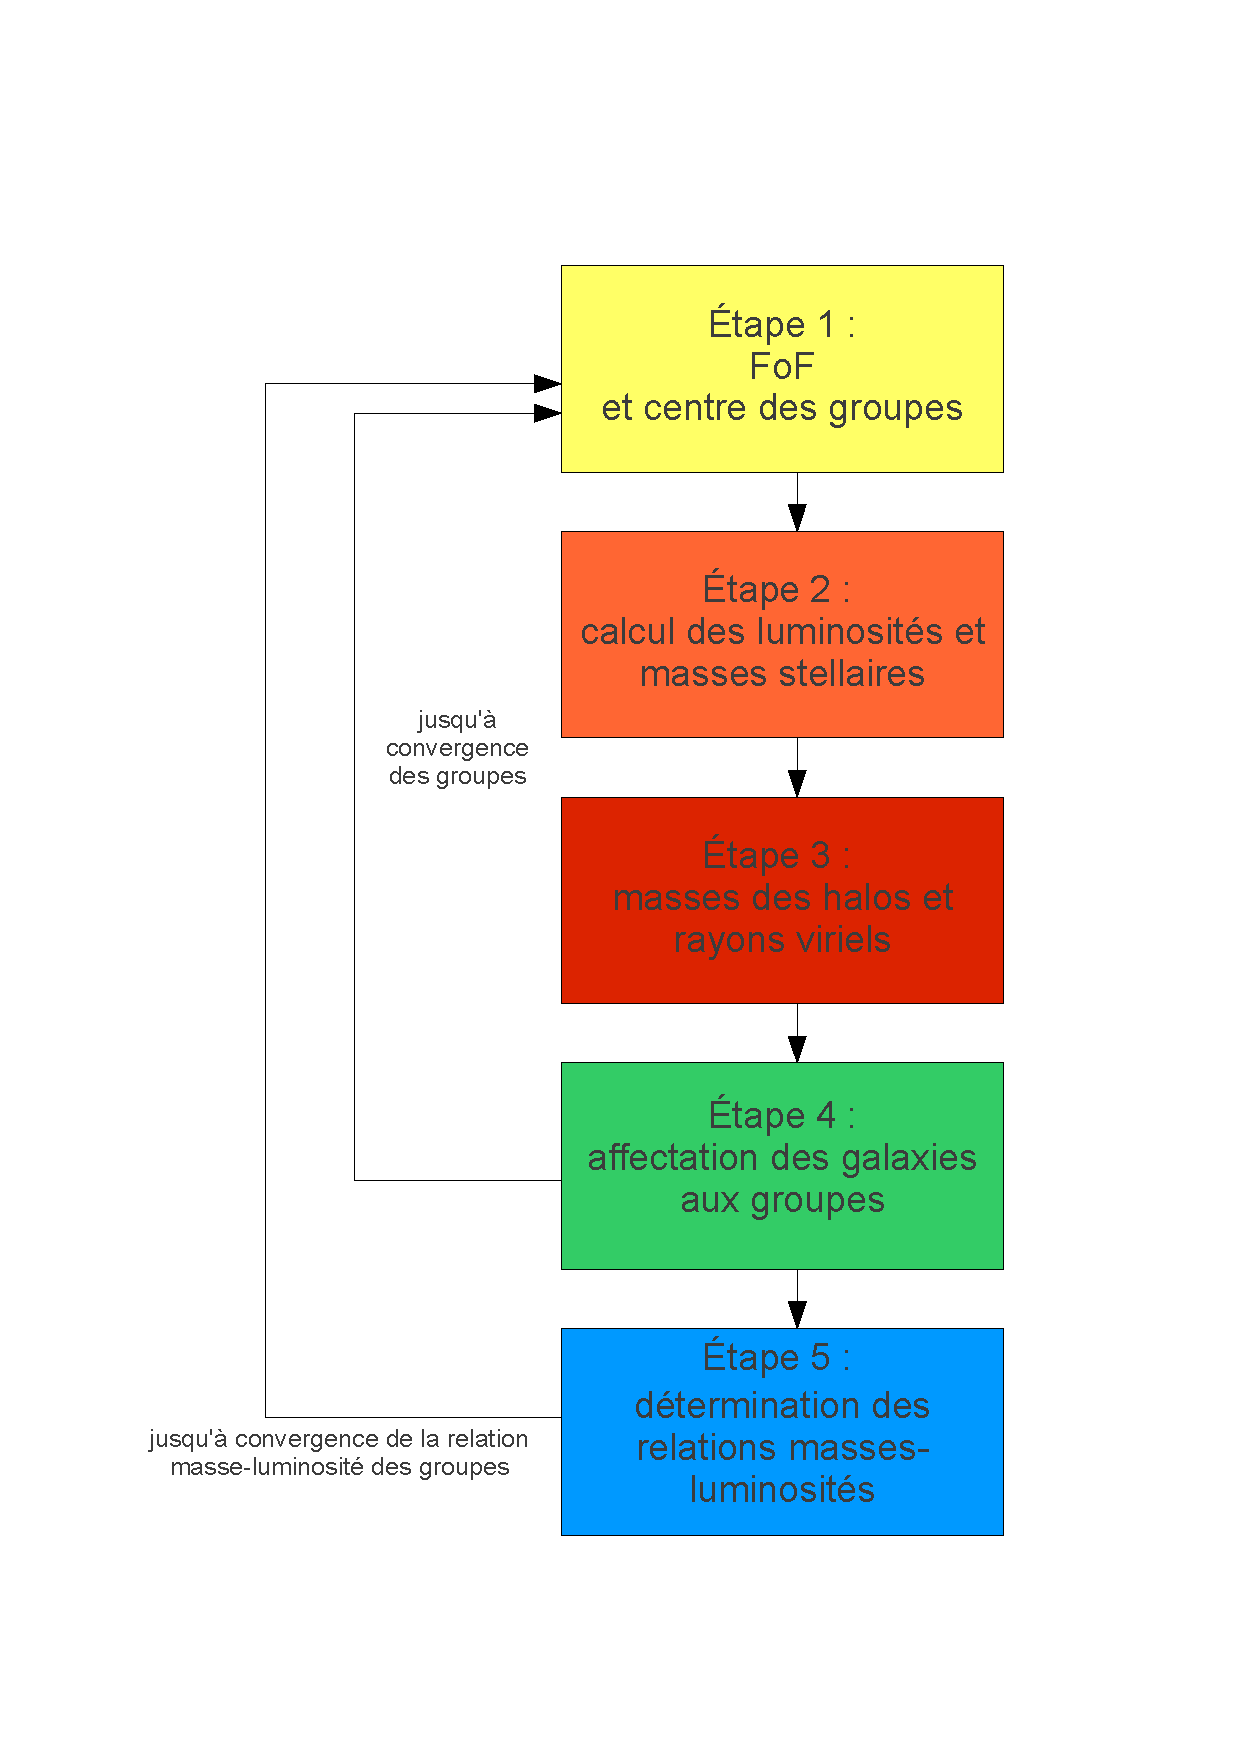
\includegraphics[width=0.5\linewidth]{org}
	\caption{\footnotesize{}Diagramme résumant les étapes de l'algorithme de \citet{Yang+07}. Les flèches représentent les
	itérations à réaliser et le texte à côté le critère d'arrêt de ces itérations.}
	\label{fig:diag}
\end{figure}

Les méthodes développées pour correspondre à l'algorithme du \citet{Yang+07} vont être décrites dans les parties suivantes.
\fss{Algorithme de Friends-of-Friends\label{sec:fof}}
L'étape \eent{1} du \citet{Yang+07} est la réalisation d'un FoF qui va permettre de trouver des groupes potentiels de galaxies pour
ensuite les mettre à jour par des itérations successives. Il a fallu alors réaliser l'algorithme du FoF. On va décrire dans la
suite le principe du FoF et le travail réalisé pour le faire fonctionner.
\fsss{Principe}
La technique du FoF n'est pas utilisée uniquement pour les groupes de galaxies de manière générale, mais essentiellement dans les
simulations cosmologiques pour identifier les halos de particules de matière noire. Le principe va donc être expliqué à partir de
ces simulations sans perte de généralité dans le cas des galaxies.

Dans les simulations, les halos sont identifiés d'abord de manière brutale par le FoF. Celui-ci considère que toutes les particules
qui ont une voisine en commun de façon directe ou indirecte font partie du même halo. On peut voir ceci illustré sur la figure
(\ref{fig:fof}). Deux particules sont considérées voisines si la distance entre elles est plus petite qu'un seuil $\epsilon$.
\begin{figure}[htb]
	\centering
	\includegraphics[width=0.5\linewidth]{fof.png}
	\caption{\footnotesize{}Relation du Friends-of-Friends: sur la figure, $A$ est liée à $C$ même si elles
	ne sont pas directement voisines, mais indirectement par l'intermédiaire de $B$ qui est
	voisine de $A$ et de $C$. Ces trois particules font partie du même groupe. Par contre $D$
	n'est liée d'aucune façon à $A,B$ ou $C$: $D$ appartient à un autre groupe.}
	\label{fig:fof}
\end{figure}

La première idée qui vient à l'esprit pour mettre en {\oe}uvre un tel algorithme est de définir deux tableaux: le premier constitué
des identités des $N$ particules de la simulation allant donc de 1 à $N$ et un second tableau de même dimension que le précédent
contenant les identités des groupes des particules. Si on n'a aucun a priori sur la structure des particules, ce second tableau est
initialisé de la même façon que le premier: chaque particule est son propre groupe. La méthode naïve qui suit est de calculer pour
chaque particule lesquelles sont voisines de celle-ci (ce qui évolue en $N^2$) et ensuite de changer les identités des groupes des
particules qui sont voisines ou liées indirectement (celles qui ont la même identité de groupe que la particule qui est voisine) ce
qui évolue, si on considère que $M$ opérations d'union sont à réaliser, en $MN$. Pour le cas du SDSS ou de notre mock catalogue,
cela peut prendre un temps considérable (plus d'un demi-million de galaxies). On a alors utilisé des méthodes qui permettent de
gagner un important temps de calcul. Pour unir les groupes qui ont une galaxie commune, on a utilisé la méthode de l'Union-Find.

\fsss{L'Union-Find}
Cette technique peut être bien comprise si on la visualise en une structure d'arbre. Dans les deux tableaux précédents le premier
contient les identités des particules qui apparaissent sur les pastilles de la figure (\ref{fig:arbre1}) et les identités des
groupes sont matérialisées par les liens entre les pastilles, l'identité de la particule à laquelle une autre est liée étant
inscrite sur la pastille supérieure à laquelle elle est liée. Par exemple sur la figure (\ref{fig:arbre1}), la particule 2 est liée
à la 5 et possède comme numéro de groupe 5, et la 8 est liée à la 2 et possède comme numéro de groupe 2. La particule 1 est isolée.
\begin{figure}[htb]
	\centering
	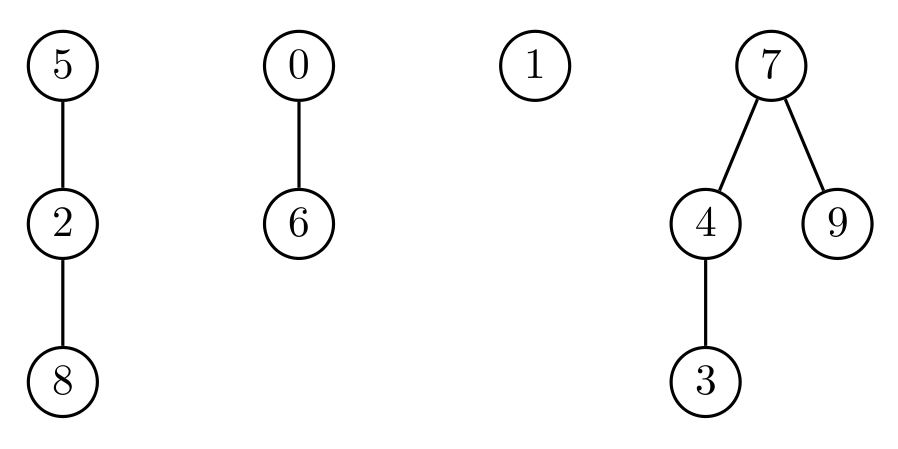
\includegraphics[width=0.5\linewidth]{arbre1.png}
	\caption{\footnotesize{}Représentation en arbre des liens entre les différentes particules.}
	\label{fig:arbre1}
\end{figure}

Pour gagner du temps de calcul, on vérifie si deux particules sont déjà liées ou non en remontant à la racine de l'arbre pour voir
si les identités diffèrent (pas encore liées) ou si elles sont identiques (déjà liées). On effectue la suite du travail si elles ne
sont pas déjà liées. Ensuite pour lier entre eux deux groupes il est plus intéressant de lier celui qui contient le moins de
membres à celui qui en contient le plus, c'est pourquoi on utilise un troisième tableau qui contient le nombre de membres de chaque
groupe (initialisé à 1 au départ) et nous permet de choisir quel groupe il faut lier en pondérant par leur taille. On peut voir le
résultat sur la figure (\ref{fig:arbre2}) de l'union pondérée de 5 et 0 de la figure (\ref{fig:arbre1}).
\begin{figure}[htb]
	\centering
	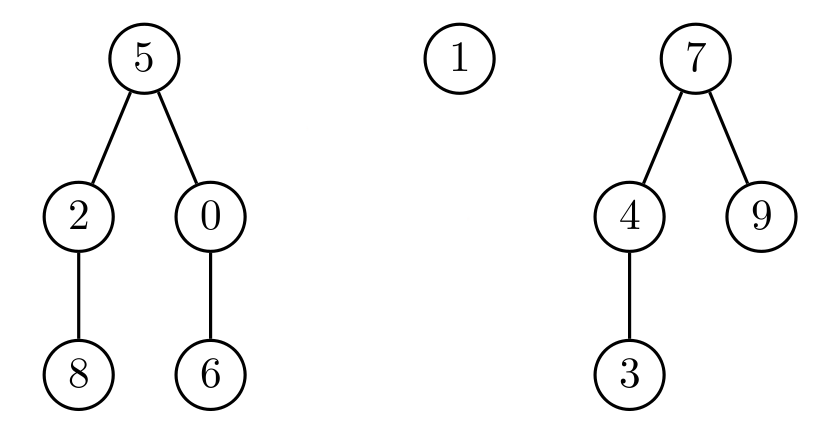
\includegraphics[width=0.5\linewidth]{arbre2.png}
	\caption{\footnotesize{}Résultat après l'union pondérée de 5 et 0 de la figure (\ref{fig:arbre1}).}
	\label{fig:arbre2}
\end{figure}
Une fois que toute la recherche des voisins est terminée et que les liens ont été établis, il est nécessaire d'aplanir les arbres
en liant directement chaque particule à la racine à laquelle elle est liée directement ou indirectement. Pour cela on remonte
chacune des branches des arbres en liant directement la particule à sa racine. On peut voir l'application de cette méthode sur la
figure (\ref{fig:arbre3}).
\begin{figure}[htb]
	\centering
	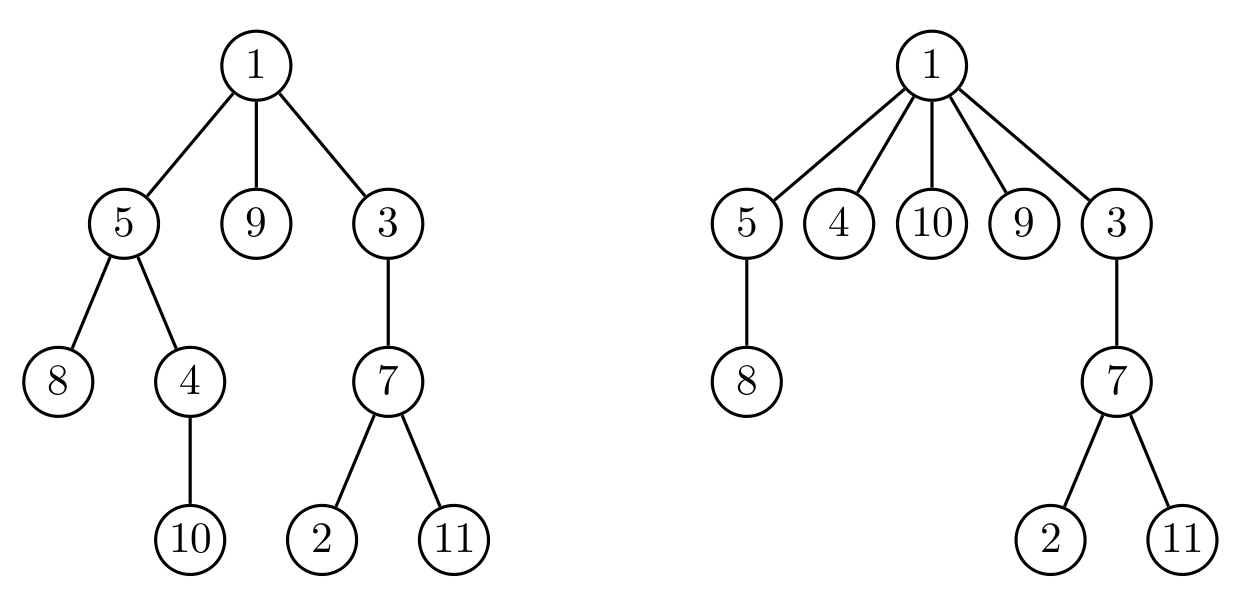
\includegraphics[width=0.5\linewidth]{arbre3.png}
	\caption{\footnotesize{}Résultat de la compression d'une branche en trouvant la racine de 10 et ensuite
	en liant (compressant) chaque n{\oe}ud de la branche rencontré en le remontant à sa racine.}
	\label{fig:arbre3}
\end{figure}
L'implémentation de cette méthode permet de gagner un précieux temps de calcul car cet algorithme évolue en $(M+N)\log{N}$ ce qui
est quasi linéaire, le $\log$ étant presque comme une constante pour ces valeurs de $N$.

Bien qu'ayant diminué le temps de calcul par cette méthode, il reste le problème de la recherche des voisins qui se réalise
toujours en $N^2$ avec la façon simple.
\fsss{Recherche des voisins}
Le coût prohibitif de temps de calcul des voisins est causé par le fait que l'on a aucune connaissance du voisinage d'une particule
qui pourrait nous faire diminuer le nombre d'opérations à effectuer, ce qui oblige à visiter chaque particule. On va donc essayer
de structurer le voisinage des particules pour limiter le nombre de calculs à réaliser.

Une façon de le faire est de subdiviser la sphère céleste en boîtes délimitées par les méridiens comme on peut le voir sur la
figure (\ref{fig:sphere}). On reproduit ce même découpage à différents niveaux en redshift, ce qui permet de créer des boîtes en 3D
sur la sphère. Ce découpage est régulier sur ($\alpha,\delta$) et sur les redshift. On place ensuite chaque galaxie dans chaque
boîte ainsi réalisée. Lors de la recherche des voisins, on prend chaque galaxie et on recherche ses voisins dans sa propre boîte et
les boîtes voisines au cas où la galaxie serait proche d'un bord de cette boîte. Le choix de la taille de la boîte est un paramètre
important car si elle plus petite que le seuil de distance qui définit que l'on est voisin ou non entre galaxies, il faut visiter
plus d'une boîte dans le voisinage de celle de la galaxie dans une direction donnée. Pour être certain de ne pas rater de galaxies
voisines, la taille des boîtes est définie à trois fois le seuil de distance à $z$ proche de zéro. Sur la figure
(\ref{fig:sphere}), on peut voir un autre problème de notre découpage en méridien: lorsqu'on s'approche du pôle céleste, si une
galaxie s'y trouve, il faut rechercher sur l'ensemble des boîtes voisines car la distance angulaire entre deux boîtes est beaucoup
plus faible. Pour prendre en compte cet effet de rapprochement entre les boîtes avec la proximité aux pôles, le nombre de boîtes à
visiter est déterminé en fonction de $\cos\delta$.

Bien que cette méthode ait des lacunes, en pratique elle permet de diminuer fortement le temps de calcul alloué à la recherche des
voisins, ce qui fait que le programme peut se dérouler assez rapidement malgré le nombre d'itérations qui peut être important. Il
ne reste plus qu'à vérifier que le programme qui a été créé donne de bons résultats sur des simulations déjà analysées.
\begin{figure}[htb]
	\centering
	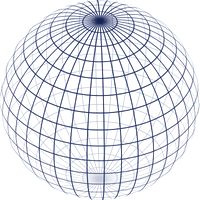
\includegraphics[width=0.3\linewidth]{sphere.jpg}
	\caption{\footnotesize{}Image illustrant le découpage de la sphère en méridien, la même chose étant
	reproduite sur plusieurs couches de redshift.}
	\label{fig:sphere}
\end{figure}
\fsss{Vérification}
Pour faire la vérification de l'algorithme de FoF, nous avons utilisé un fichier contenant les positions de particules de matière
noire issues d'une simulation de \num{64^3} particules. Ces données ont été fournies par Thierry SOUSBIE qui avait déjà réalisé un
FoF dessus et on connaissait donc déjà les résultats à l'avance. Ce fichier contient aussi les informations permettant de retrouver
les groupes de plus de \num{100} particules. Il nous a indiqué qu'il y \num{799} groupes de plus de \num{20} membres. Avec notre
programme, on trouve 801 groupes dans ce cas là. Pour être plus sûr des résultats, on a réalisé la distribution en nombre de
membres par groupe, c'est-à-dire l'histogramme du nombre de membres par groupes. La comparaison a indiqué que les distributions
fournies par les données du fichier et notre programme sont sensiblement identiques: les plus gros groupes sont bien retrouvés mais
quelques différences persistent avec des variations de un ou deux membres pour une quinzaine de groupes. Pour être certain de la
méthode de l'Union-Find utilisée, on a utilisé aussi la méthode simple mais plus longue qui a été décrite plus haut. Les résultats
obtenus sont identiques.

Après discussion avec Thierry SOUSBIE, il s'avère que le fichier fourni n'a pas la même précision pour les positions des particules
que celle utilisée pour générer les données de ce fichier. Il est donc normal de trouver des résultats légèrement différents que
ceux qui nous sont fournis. Si à cause de cette perte de précision dans les calculs, une particule ne se trouve plus voisine d'une
autre, il se peut qu'elle soit voisine d'une autre particule avec laquelle elle n'est pas liée quand la précision des données est
plus élevée. Ceci peut bouleverser complètement la structure déterminée par notre programme par rapport à celle réelle. Cela
explique aussi les différences d'une ou deux particules observées pour les groupes trouvés par les deux programmes.

Du fait que la méthode simple, plus longue mais plus sûre, donne les mêmes résultats que la méthode rapide permet de dire que cet
algorithme fonctionne bien, les différences étant imputables à la précision des données du fichier de test par rapport à la
précision à laquelle elles ont été générées. Maintenant nous sommes certains du bon fonctionnement de cette partie du programme et
on peut commencer à implémenter le reste de l'algorithme de \citet{Yang+07}.
\fss{Réalisation du Yang \textit{et al.}}
Les méthodes mises en {\oe}uvre pour chaque étape du Yang \textit{et al.} vont maintenant être détaillées.
\fsss{\'Etape 1: centre des groupes FoF préliminaires\label{sec:et1}}
L'algorithme de FoF a été mis en place, il reste à choisir le paramètre de lien pour le réaliser. Dans l'article il est indiqué
qu'on choisit un lien de $l_p$=\num{0,05} selon la direction transverse à la ligne de visée et de $l_z$=\num{0,3} en unité de
séparation moyenne des galaxies au redshift en question. En effet cette séparation varie avec le redshift et il faut donc la
déterminer. On la calcule à l'aide de la densité comobile de galaxies. Elle s'exprime ainsi:
\begin{eq}
        n(z)=\int_{L_{\rm{min}}(z)}^{\infty}\phi{(L)}\dd{L}\label{eq:dens}
\end{eq}
avec $\phi{(L)}$ la fonction de luminosité différente selon le cas où on traite le mock catalogue ou le SDSS. Le choix de cette
fonction de luminosité est important car elle doit traduire au mieux les propriétés du catalogue de galaxie que l'on considère afin
d'estimer correctement la séparation moyenne des galaxies. Dans \citet{Guo+11}, il est indiqué que la fonction de luminosité
utilisée pour réaliser les simulations du mini-MSII correspondent assez bien aux données du SDSS utilisées dans \citet{Blanton+05}.
Afin de vérifier, que cela est vrai on a réalisé la fonction de luminosité du mini-MSII et on l'a comparée à celle donnée dans
\citet{Blanton+05}. Il s'avère qu'il y a quelques différences qui peuvent jouer de façon importante dans cette estimation de la
séparation moyenne. C'est pourquoi on a essayé de modéliser la fonction de luminosité de \citet{Guo+11} par une interpolation par
splines cubiques, après avoir tenté différentes approches pour cette modélisation comme l'ajustement par des polynômes de
différents ordres de la fonction de luminosité et également par des fonctions de Schechter avec des paramètres obtenus par la
méthode du maximum de vraisemblance. Il résulte de cette modélisation par splines cubiques qu'elle permet d'ajuster de façon très
précise les données du Guo2010a.

La fonction de luminosité des données du Guo2010a est tracée sur la figure (\ref{fig:lumfonc}) (en orange) avec celle obtenue par
les splines cubiques (en rouge) et celle de \citet{Blanton+05} (en vert). On remarque bien que l'ajustement à l'aide des splines
cubiques donne de bons résultats, meilleurs que ceux de \citet{Blanton+05}. L'intégrale de cette fonction de luminosité pour
obtenir la densité de galaxies ne sera fera alors pas jusqu'à l'infini mais jusqu'à la magnitude qui correspond à la galaxie la
plus lumineuse du catalogue Guo2010a (qui est la valeur limite visible sur la figure (\ref{fig:lumfonc}).
\begin{figure}[htb]
	\centering
	\includegraphics[width=0.5\linewidth]{lumfonc.pdf}
	\caption{\footnotesize{}Comparaison des différentes fonctions de luminosités: la fonction représentée en orange est celle
	déterminée à partir des données du catalogue Guo2010a du mini-MSII, celle en vert les données de la fonction obtenues à
	partir de \citet{Blanton+05} et celle en rouge l'ajustement par les splines cubiques que l'on a appliqué.}
	\label{fig:lumfonc}
\end{figure}

Dans le cas du SDSS, on va adopter comme fonction de luminosité celle de \citet{Blanton+05} car elle permet de modéliser de façon
optimale les données du survey SDSS. Il ne reste plus qu'à déterminer la luminosité limite en fonction du redshift pour estimer la
séparation moyenne entre galaxies. On sait que la magnitude apparente limite du SDSS est \num{17,77} en bande $r$, et on la note
$m_{\rm{lim}}$. La luminosité limite à un redshift donné traduit la magnitude absolue maximale des galaxies observées à ce redshift
$M_{\rm{lim}}$ et on peut écrire:
\begin{eq}
        M_{\rm{lim}}=m_{\rm{lim}}-5\logg\left(\frac{d_{\rm{lum}}}{10pc}\right)
\end{eq}
Donc la luminosité limite peut s'écrire:
\begin{eq}
        L_{\rm{lim}}(z)={{\left(\frac{d_{\rm{lum}}}{10pc}\right)}^2}\num{10}^{\num{0.4}(M_{\odot}-m_{\rm{lim}})}
\end{eq}
où la dépendance en $z$ se fait par l'intermédiaire de la distance lumineuse. Théoriquement pour réaliser les calculs précisement
on devrait prendre en compte les effets de la correction-K sur cette luminosité limite qui dépend aussi de l'allure du spectre de
la galaxie donc de son type et de sa couleur. Mais pour faciliter le travail et les calculs à réaliser, on se passera de cette
précision sur la luminosité limite, sinon il aurait fallu déterminer une correction-K moyenne en fonction du redshift afin de
prendre en compte cet effet, ce qui n'est pas précis également.

Pour vérifier que cette méthode donne de bons résultats, on va essayer de réaliser un comptage des galaxies dans notre mock
catalogue et le comparer à un calcul théorique pour voir les différences qui peuvent apparaître et influencer le calcul de la
séparation moyenne dans le FoF. La densité comobile de galaxies peut s'exprimer sous cette forme également:
\begin{eq}
        n(z)=\frac{\dd{N}}{\dd{z}}\frac{\dd{z}}{\dd{V}}
\end{eq}
où $\dd{N}$ est le nombre de galaxies dans un intervalle de $\dd{z}$ et $\dd{V}$ le volume comobile élémentaire de calcul.
$\dd{N}/\dd{z}$ peut être déterminé par comptage des galaxies par intervalles de redshift directement à partir des données.
$\dd{V}$ peut s'exprimer comme:
\begin{eq}
        \dd{V}={D_{\rm{H}}}\frac{{(1+z)}^2{D_{\rm{A}}}^2}{E(z)}{\dd{\Omega}}{\dd{z}}
\end{eq}
avec ${D_{\rm{A}}}$ la distance angulaire, $D_{\rm{H}}=c/{H_0}$ et $d\Omega$ l'angle solide dans lequel on réalise le comptage. La
distance angulaire s'exprime en fonction de la distance lumineuse comme:
\begin{eq}
        {D_{\rm{A}}}=\frac{d_{\rm{lum}}}{(1+z)^2}
\end{eq}
La fonction $E(z)$ est le rapport de la constante de Hubble à un $z$ donné par rapport à $z=0$. Elle s'exprime (dans le cas d'un
Univers plat) comme:
\begin{eq}
        E(z)=\sqrt{\Omega_{m}(1+z)^3+\Omega_{\Lambda}}
\end{eq}
où $\Omega_{m}$ représente la fraction de la matière dans l'Univers et $\Omega_{\Lambda}$ la part de l'énergie noire, avec
$\Omega_{m}+\Omega_{\Lambda}=\num{1}$. En utilisant à nouveau l'approximation pour la distance lumineuse donnée par \citet{WU10},
on peut déterminer facilement $\dd{N}/\dd{z}$ de façon théorique avec les expressions de $n(z)$ basées sur les fonctions de
luminosité. Les résultats sont présentés sur la figure (\ref{fig:dN_dz}) pour un mock catalogue où aucune correction-K n'a été
appliquée sur les galaxies. Ainsi le calcul théorique de $\dd{N}/\dd{z}$ doit coller parfaitement avec le comptage réalisé sur le
mock catalogue, aucune perte de galaxies par un biais quelconque ne devant se produire dans le mock catalogue. Sur la figure
(\ref{fig:dN_dz}) les résultats à partir du mock catalogue non K-corrigé et sans prise en compte des vitesses particulières pour
les redshifts sont en bleu et notre calcul théorique en violet. Les résultats sont très similaires pour les deux courbes, les
fluctuations visibles sur la courbe bleue étant causées par des variations locales de la densité de galaxies dans le mock (la
répartition en filaments des galaxies y étant pour une grande partie responsable). On voit aussi une divergence entre les deux
courbes aux grands redshifts, causées par une mauvaise estimation du nombre de galaxies avec une luminosité élevée (seules visibles
à ces grandes distances) à cause de notre de choix de magnitude limite pour la borne supérieure de l'intégrale de l'équation
(\ref{eq:dens}) qui est un peu arbitraire et du bruit dans la fonction de luminosité en orange sur la figure (\ref{fig:lumfonc})
qui donne une moins bonne évaluation par les splines cubiques et donc une valeur de l'intégrale moins précise.
\begin{figure}[htb]
	\centering
	\includegraphics[width=0.5\linewidth]{dN_dz.pdf}
	\caption{\footnotesize{}Comptage des galaxies par intervalle de redshift: en bleu les résultats obtenus directement à
	partir de notre mock catalogue (sans correction-K ni vitesse particulière), en mauve le calcul théorique détaillé dans le
	rapport.}
	\label{fig:dN_dz}
\end{figure}

On fait le même travail pour un mock catalogue avec cette fois une correction-K appliquées à chaque galaxie et des vitesses
particulières pour calculer les redshifts comme décrit dans la section (\ref{sec:galcarac}) pour voir l'effet de la correction-K
par rapport à notre estimation théorique du nombre de galaxies. Le résultat se trouve sur la figure (\ref{fig:compt}). Cette
correction réduit un petit peu le nombre de galaxies par rapport au cas précédent et s'écarte donc un peu du calcul théorique mais
pas avec des écarts important ce qui nous permet de conserver notre estimation de la densité moyenne de galaxie par les splines
cubiques dans le cas du mock catalogue.
\begin{figure}[htb]
	\centering
	\includegraphics[width=0.5\linewidth]{compt}
	\caption{\footnotesize{}Comptage des galaxies par intervalle de redshift: les résultats sont présentés de la même manière
	que la figure (\ref{fig:dN_dz}) sauf que cette fois une correction-K a été appliquée sur les galaxies du mock et les
	vitesses particulières ont été prises en compte pour la calcul des redshifts. On voit que leur considération dans le mock
	catalogue atténue un peu le nombre de galaxies disponibles dans notre mock par rapport au cas théorique où on ne prend pas
	ces effets en compte. Les différences entre les courbes théoriques avec la figure (\ref{fig:dN_dz}) sont dues à de légères
	différences entre les bornes de l'intégration pour la magnitude minimale qui influent sur les grandes luminosités (donc les
	grands redshifts), pour des facilités de calcul et ont peu d'importance étant donnée l'imprécision du calcul à ces
	redshifts.}
	\label{fig:compt}
\end{figure}

Nous pouvons maintenant déterminer la séparation moyenne entre galaxies, celle-ci étant égale à $1/{n(z)}^{1/3}$, pour connaître le
paramètre de lien entre galaxies.

Pour savoir si deux galaxies sont voisines ou non, on utilise les critères définis dans
\citet{Eke+04}. En posant $l_p$ et $l_z$ les paramètres de lien entre galaxies dans une direction transverse à la ligne de visée et
suivant la ligne de visée respectivement, on considère que deux galaxies $i,j$ sont voisines si la séparation angulaire entre les
deux galaxies $\theta_{ij}$ est telle que:
\begin{eq}
        \theta_{ij}\leq\frac{1}{2}\left(\frac{l_{p,i}}{d_{c,i}}+\frac{l_{p,j}}{d_{c,j}}\right)
\end{eq}
et si:
\begin{eq}
        |d_{c,i}-d_{c,j}|\leq\frac{l_{z,i}+l_{z,j}}{2}
\end{eq}
avec $d_c$ la distance comobile de la galaxie correspondante.

Nous avons maintenant complété l'étape \eent{1} et on peut passer à la description de l'étape \eent{2}.
\fsss{\'Etape 2: correction des luminosités}
Dans cette étape, il y a deux effets considérés: l'incomplétude de la luminosité causée par la magnitude limite du survey ainsi que
la correction provoquée par les effets de bord. Il est tout d'abord nécessaire de déterminer la fonction de correction des
luminosités pour la première itération. Elle est définie ainsi:
\begin{eq}\label{eq:corr}
        f(L_{\num{19,5}},L_{lim})=\frac{\int_{L_{lim}}^{\infty}L\phi{(L)}\dd{L}}{\int_{L_{cut}}^{\infty}L\phi{(L)}\dd{L}}
\end{eq}
avec $L_{cut}$ la luminosité correspondante à $M_r=-\num{19,5}$, luminosité de coupure de l'échantillon et $\phi(L)$ la fonction de
luminosité. Ceci permet de représenter la part de luminosité des membres effectivement dans le groupe par rapport à ce que cela
serait si le groupe était complet. Donc pour corriger de la part manquante dans la luminosité caractéristique, on multiplie par
l'inverse de cette fonction $f$.

Pour le choix de la fonction de luminosité nous avons choisie celle donnée par \citet{Blanton+05} qui modélise au mieux les données
du SDSS. La fonction s'exprime ainsi:
\begin{eq}
        \phi(L)\dd{L}=\frac{\dd{L}}{L_*}\exp\left(-\frac{L}{L_*}\right)\left[\phi_{*,1}\left(\frac{L}{L_*}\right)^{\alpha_1}+
        \phi_{*,2}\left(\frac{L}{L_*}\right)^{\alpha_2}\right]
\end{eq}

Les valeurs des paramètres sont listées dans le tableau (\ref{tab:paramblan}). Quand on injecte cette fonction de luminosité dans
l'équation (\ref{eq:corr}), on voit que la fonction de correction peut s'exprimer comme une somme de fonction gamma incomplète
$\Gamma(a,x)=\int_x^{\infty}t^{a-1}e^{-t}dt$ et on peut donc écrire:
\small
\begin{eq}
        f(L_{\num{19,5}},L_{lim})=\frac{\phi_{*,1}\Gamma(2+\alpha_1,\frac{L_{lim}}{L_*})+\phi_{*,2}\Gamma(2+\alpha_2,\frac{L_{lim}}{L_*})}
        {\phi_{*,1}\Gamma(2+\alpha_1,\frac{L_{cut}}{L_*})+\phi_{*,2}\Gamma(2+\alpha_2,\frac{L_{cut}}{L_*})}
\end{eq}
\normalsize
\begin{table}[htb]
	\centering
	\begin{tabular}{>{\columncolor{bleu2}}c>{\columncolor{bleu3}}c>{\columncolor{bleu2}}c>{\columncolor{bleu3}}c>{\columncolor{bleu2}}c}
	\hline
		$M_*-5\logg{h}$           & $\phi_{*,1}$               & $\alpha_1$               & $\phi_{*,1}$               & $\alpha_2$ \\
                            & (\num{e-2}${h^3}{Mpc^{-3}}$) &                          & (\num{e-2}${h^3}{Mpc^{-3}}$) & \\ \hline
		\num{-20.04}$\pm$\num{0.03} & \num{1.56}$\pm$\num{0.05}    & \num{-0.17}$\pm$\num{0.07} & \num{0.62}$\pm$\num{0.04}    & \num{-1.52}$\pm$\num{0.01} \\ \hline
	\end{tabular}
	\caption{\footnotesize{}Les paramètres de la fonction de luminosité de \citet{Blanton+05} utilisés dans notre cas.}
	\label{tab:paramblan}
\end{table}

Pour réaliser le calcul de cette fonction $\Gamma$ incomplète, on a utilisé la procédure qui est décrite en
annexe (\ref{sec:anngam}) qui réalise le calcul de manière rapide.

Dans le cas du mock catalogue, on utilise aussi la fonction de luminosité calculée directement à partir des données du Guo2010a et
on ajuste à l'aide des splines cubiques la fonction $L\phi(L)$ qu'on doit intégrer de la même façon que précédemment. Ce type de
calcul pour la fonction $f$ n'est réalisé que pour la première itération suivant le FoF ou la détermination d'une relation
masse-luminosité ainsi que celle de la fonction de correction elle-même. La façon dont on détermine cette fonction de correction
pour les autres itération sera décrite plus loin.

Le \citet{Yang+07} permet également de déterminer les masses stellaires des groupes de galaxies à partir des masses stellaires des
galaxies déterminées par l'équation (\ref{eq:mstel}). Le principe de la détermination des masses stellaires des groupes est la même
sur le principe que pour la luminosité des groupes sauf que la fonction de correction notée $g$ dans ce cas là n'est pas déterminée
pour la première itération mais on utilise seulement la relation déduite pour chaque itération décrite plus loin.

Un autre effet important doit être pris en compte à cette étape: c'est l'effet de bord. Certains groupes que l'on détermine sont
situés au bord soit du mock catalogue soit du survey pour le SDSS. Ceci peut faire en sorte que certains groupes aient des galaxies
manquantes dans leur membres, ce qui se traduit pas une mauvaise évaluation de leurs propriétés. Il faut donc prendre en compte cet
effet. Pour cela le principe est à peu de choses près le même pour le mock et pour le SDSS. On recherche d'abord les groupes qui
sont susceptibles d'avoir des galaxies manquantes parce qu'ils sont situés aux bords, donc les groupes qui ont la position de leur
rayon de Viriel qui sort du mock peuvent avoir des galaxies manquantes (une partie de la sphère virielle se retrouve en-dehors du
mock), et pour le SDSS il s'agit des groupes qui sont à une complétude $\mathcal{C}>\num{0,7}$ dans leur sphère virielle. Une fois
ces groupes trouvés, on distribue aléatoirement \num{200} points dans la sphère virielle du groupe et tous les points qui sortent
alors du groupe (par leur position pour le mock et par la complétude pour le SDDS) sont supprimés. On peut voir cela sur la figure
(\ref{fig:effetbord}) où on a représenté un groupe dont la sphère virielle sort de la zone du mock délimitée par le plan en vert.
Les points qui sont placés aléatoirement sont en jaune s'ils sont sortis du mock et en bleu s'ils sont dans les limites du
catalogue. On détermine pour chaque groupe le nombre de points restant parmi les \num{200} noté $N_{\rm{restant}}$ et on définit
$f_{\rm{edge}}=N_{\rm{restant}}/\num{200}$ comme la part du volume du groupe qui repose dans le catalogue. La fraction des galaxies
manquantes dans les propriétés des groupes (luminosité et masse stellaire) est alors corrigée en ajoutant un facteur de correction
$1/f_{\rm{edge}}$ quand on estime la luminosité et les masses stellaires comme dans le cas où le groupe est incomplet. Cependant
ceci ne fonctionne pas bien pour les groupes avec un $f_{\rm{edge}}$ petit donc on élimine les groupes avec
$f_{\rm{edge}}<\num{0,6}$.
\begin{figure}[htb]
	\centering
	\includegraphics[width=0.3\linewidth]{effetbord}
	\caption{\footnotesize{}Représentation de l'effet de bord des groupes. La sphère virielle est représentée en rouge et la
	bordure du catalogue par le plan en vert. Les points placés aléatoirement dans la sphère virielle sont jaunes s'ils sont en
	dehors du catalogue et sont en bleu s'ils sont dans les limites du catalogue. Cette image n'est valable que pour le mock
	catalogue qui a des bordures nettes alors que pour le SDSS, il faut utiliser l'incomplétude du survey $\mathcal{C}$.}
	\label{fig:effetbord}
\end{figure}

\fsss{\'Etape 3: masses et rayons des groupes}
Cette étape nécessite de déterminer la masse du halo associé au groupe trouvé précédemment. Pour cela on utilise une relation
masse-luminosité fixée au départ, puis on utilise la relation que l'on détermine aux itérations suivantes. La méthode pour la
déterminer sera décrite elle aussi plus loin.
\fsss{\'Etape 4: appartenance des galaxies}
On doit calculer à cette étape la densité de contraste qui nous sert à définir un critère d'appartenance d'une galaxie à un groupe.
Pour cela on doit pour chaque galaxie boucler sur les groupes et calculer la distance projetée au centre du groupe, au redshift du
groupe. Si on réalise le calcul de cette façon, le même problème que celui décrit plus haut sur le temps nécessaire se pose. On
procède alors là aussi à un découpage de la sphère céleste pour accélérer cette recherche. La taille des boîtes dans ce cas est
choisie plus grande pour ne pas introduire de sélection des galaxies, leur appartenance au groupe dépendant maintenant d'un critère
qui n'est pas défini seulement par la distance au centre du groupe. En prenant des boîtes "larges" pour le découpage, on supprime
les effets de sélection. Le découpage réalisé dans ce cas n'est pas le même que celui réalisé pour le FoF, la taille des boîtes
étant conservées à peu près constante pour chaque bin en redshift et quand on fait varier la déclinaison $\delta$ et l'ascension
droite $\alpha$. La structure résultante n'est pas alors aussi simple que celle de la figure (\ref{fig:sphere}) et des précautions
supplémentaires ont été appliquées pour éviter de manquer des boîtes dans la recherche des groupes auxquels une galaxie peut
appartenir. Les boîtes ont été choisies larges dans le sens des redshifts afin de prendre en compte les effets d'élongation évoqués
dans la section (\ref{sec:elong}). Une image qui pourrait convenir est celle de la figure (\ref{fig:dec}). On voit que dans ce cas
le maillage n'est pas régulier. Les boîtes représentent le découpage dans l'espace projeté (sphère céleste) et les redshifts. Comme
on essaie de garder des boîtes de taille constante dans l'espace physique, cela se traduit par un nombre de boîtes plus important
aux grands redshifts qu'aux petits. Et étant donnée la géométrie sphérique du problème, pour une boîte où on cherche les groupes
potentiels d'une galaxie, il faut chercher dans un plus grand nombre de boîtes sur l'extrémité en $z$ où $z$ est le plus grand que
sur celle ou $z$ est plus faible. C'est ce qu'on tente de représenter sur la figure (\ref{fig:dec}) où les différentes tranches de
redshift ont des boîtes colorées différemment. Pour représenter le nombre de boîtes à visiter pour la galaxie située dans la boîte
rouge qui est croissant avec le redshift, la taille des boîtes a été diminué quand $z$ augmente (la taille des boîtes en angle
diminue au fur et à mesure que l'on s'éloigne de l'observateur). Si on se place dans la boîte rouge en tant que galaxie et que l'on
cherche les groupes voisins, il faut chercher dans les boîtes adjacentes seulement pour un $z$ donné (les boîtes orange), par
contre les boîtes juste inférieures et supérieures en redshift sont en contact de manières différentes selon les situations avec la
boîte rouge. La recherche des groupes voisins dans les boîtes voisines n'est alors pas très aisée: on a donc décidé de rechercher
dans les 5 boîtes voisines en $\alpha$ et pour chaque étage en $\delta$ dans le but de limiter le nombre de recherche tout en
estimant que l'on ne manque aucun groupe en prenant de cette façon \emph{large} dans les boîtes voisines (ce qu'on peut voir
également sur la figure (\ref{fig:dec}) sur la vue de face où on prend en compte toutes les boîtes voisines en appliquant ce
traitement). On estime donc que la méthode mise en {\oe}uvre permet d'optimiser le programme en diminuant fortement le temps de
calcul tout en permettant d'effectuer une recherche des groupes voisins sûre.
\begin{figure}[p]
	\centering
	\begin{minipage}{\linewidth}
	\subfloat[Vue de côté]{
	\includegraphics[width=0.49\linewidth]{dec1}}
	\subfloat[Vue de face]{
	\includegraphics[width=0.49\linewidth]{dec2}}
	\end{minipage}
	\begin{minipage}{\linewidth}
	\subfloat[Vue de dessous]{
	\includegraphics[width=0.49\linewidth]{dec3}}
	\subfloat[Vue arrière]{
	\includegraphics[width=0.49\linewidth]{dec4}}
	\end{minipage}
	\caption{\footnotesize{}Illustration du découpage de la sphère céleste dans un maillage non régulier. La flèche bleue
	foncée représente l'axe croissant des redshifts, la flèche bleue claire l'ascension droite $\alpha$ et la flèche violette
	la déclinaison $\delta$. La boîte rouge au centre représente la boîte où se trouve la galaxie dont on cherche les groupes
	auxquels elle pourrait appartenir. Les quatre figures représentent le même dessin mais vu de plusieurs points de vue
	différents pour aider à la visualisation en 3D du découpage. Il faut garder à l'esprit qu'il s'agit d'une représentation
	par des cubes de sections de cône, mais cela est sensiblement identique quand le nombre de boîtes est élevé pour le
	découpage et que l'on regarde seulement un petit morceau de la sphère.}
	\label{fig:dec}
\end{figure}

Comme décrit dans la section (\ref{sec:et4}), on doit calculer la concentration $c_{180}=r_{180}/r_s$, mais on ne connaît pas $r_s$
a priori. Donc pour déterminer ce rayon caractéristique, on va utiliser les résultats établis par \citet{MDvdB08} pour calculer la
concentration. On se base sur les résultats obtenus pour une cosmologie WMAP5 qui donnent:
\begin{eq}
        \log_{10}c_{200}=\num{0,830}-\num{0,098}\log_{10}\left(\frac{M_{200}}{\num{e12}h^{-1}M_{\odot}}\right)
\end{eq}
Or nous avons besoin des résultats avec $c_{180}$, on va donc appliquer quelques corrections à ces résultats pour déterminer $r_s$.
D'une manière qui ne sera pas décrite ici, on peut déterminer le rapport $r_{180}/r_{200}$ qui varie peu avec la concentration et
de la même façon le rapport des masses $M_{180}/M_{200}$. On obtient pour ces rapports:
\begin{eqnarray}
        \log_{10}\left(\frac{M_{180}}{M_{200}}\right)&\approx&\num{0,012}\nonumber\\
        \rm{et}\hspace{5pt}\log_{10}\left(\frac{r_{180}}{r_{200}}\right)&\approx&\num{0,019}\nonumber\\
\end{eqnarray}
Il nous suffit maintenant de déterminer l'expression de $M_{180}$ afin de pouvoir obtenir une valeur de $c_{180}$. En notant
$\Delta$ la sur-densité de l'Univers, et $\rho_c$ la densité critique, on a:
\begin{eq}
        M_{180}=\Delta\left(\frac{4}{3}\pi{r_{180}}^3\right){\rho_c}
\end{eq}
Dans notre situation, $\Delta=\num{180}$ et en utilisant l'expression de la densité critique:
\begin{eq}
        M_{180}=\frac{\num{90}{{H_0}^2}{{r_{180}}^3}}{G}
\end{eq}
Tout ceci permet finalement d'écrire:
\begin{eq}
        \log_{10}c_{180}=\num{0.849}-\num{0.098}\log_{10}\left(\frac{\num{90}{{H_0}^2}{{r_{180}}^3}}{G{h^{-1}}\num{e12}{M_{\odot}}}\right)
\end{eq}
avec $G$ exprimé dans les unités appropriées.

Il reste un dernier problème à régler si on réalise comme il est décrit dans l'article le regroupement des galaxies selon le
paramètre de densité de contraste. En effet, si on considère deux galaxies proches et non encore attachées à un groupe et que le
critère permet de lier la première galaxie à la seconde (considérée comme un groupe même si elle est seule dans ce groupe) et la
seconde à la première, la simple application de la méthode décrite plus haut et dans \citet{Yang+07} donnera toujours deux galaxies
isolées (deux groupes distincts) car la première prendra l'identité du groupe de la seconde et la seconde l'ancien numéro de groupe
de la première. Finalement elles seront considérées comme appartenant à deux groupes différents alors que selon le critère de
regroupement elles peuvent appartenir au même groupe. On applique donc une vérification quand on lie une galaxie à un groupe afin
de déterminer si cette galaxie n'a pas déjà été liée à une galaxie isolée pour prévenir ainsi ces oscillations de paires. Le même
genre de situation problématique peut survenir avec des triplets (voire des multiplicités plus grandes) de galaxies isolées où
chaque galaxie peut être liée ainsi successivement à sa voisine dans une sorte de cercle vicieux. Mais on considère que ce genre de
situation a peu de chances de se produire et aucune vérification n'est réalisée pendant le regroupement pour empêcher ce type
"d'oscillations" d'appartenance aux groupes.
\fsss{\'Etape 5: itérations}
Pour déterminer les groupes avant le calcul de la fonction de correction et de la relation masse-luminosité, il faut faire une
itération sur la détermination des membres des groupes. Elle doit cesser lorsque le nombre de groupes ainsi que leur richesse en
galaxie ont peu évolués par rapport à l'itération précédente. Pour définir un critère de convergence, on va utiliser la fonction de
multiplicité des groupes, c'est-à-dire déterminer le nombre de groupes qui ont un certain nombre de galaxies comme membres. Le
critère sera proche de celui du $\chi^2$ en statistique.

Pour résumer, on cherche à savoir si le nombre de groupes avec un certain nombre de galaxies comme membres évolue peu. On dispose
donc de deux distributions de deux itérations successives. On note $N_{1i}$ le nombre de groupes de la première distribution (1)
ayant $i$ galaxies membres et $N_{2i}$ la même chose pour la seconde distribution (2). La convergence est assurée si le nombre de
groupes avec un certain nombre de galaxies membres n'évolue plus beaucoup, donc on définit le $\chi^2$ comme:
\begin{eq}
        \chi^2=\frac{1}{N_{\rm{tot}}}\sum_{i=1}^{N_{\rm{tot}}}\frac{{(N_{1i}-N_{2i})}^2}{{(N_{1i}+N_{2i})}^2}\frac{1}{{\sigma^2}
        \left(\frac{N_{1i}-N_{2i}}{N_{1i}+N_{2i}}\right)}
\end{eq}
c'est-à-dire que l'on réalise une statistique sur les $\Delta_i=\frac{|N_{1i}-N_{2i}|}{N_{1i}+N_{2i}}$, ce qui permet d'évaluer une
différence relative du nombre de groupes ayant un certain nombre de galaxies. Comme on réalise un comptage, on peut utiliser une
statistique de Poisson, donc l'écart type $\sigma$ peut se calculer comme:
\begin{eqnarray}
        \sigma^2(N_{1i})&=&N_{1i}\nonumber\\
        \sigma^2(N_{1i}\pm{N_{2i}})&=&N_{1i}+N_{2i}\nonumber\\
        \sigma^2\left(\frac{A}{B}\right)&=&\left(\frac{({A}{\sigma(B)})}{B^2}\right)^2+\left(\frac{\sigma(A)}{B}\right)^2\nonumber\\
\end{eqnarray}
On trouve alors:
\begin{eq}
        \sigma^2\left(\frac{N_{1i}-N_{2i}}{N_{1i}+N_{2i}}\right)=\frac{{(N_{1i}-N_{2i})}^2}{{(N_{1i}+N_{2i})}^3}+\frac{1}{N_{1i}+N_{2i}}\approx
        \frac{1}{N_{1i}+N_{2i}}
\end{eq}
Donc finalement le critère du $\chi^2$ se résume à:
\begin{eq}
        \chi^2=\frac{1}{N_{\rm{tot}}}\sum_{i=1}^{N_{\rm{tot}}}\frac{{(N_{1i}-N_{2i})}^2}{(N_{1i}+N_{2i})}
\end{eq}
Plus $\chi^2$ devient petit et plus les distributions sont proches l'une de l'autre. \`A partir de cela on peut voir comment se
comporte le $\chi^2$ au fur et à mesure des itérations dans un cas pour déterminer à quel moment il converge vers une valeur limite
qui servira à définir le seuil à partir duquel on stoppe les itérations. On peut voir son évolution avec les itérations sur la
figure (\ref{fig:evchi2}). Le $\chi^2$ finit par converger aux alentours d'une valeur que l'on se fixera approximativement comme
seuil pour l'arrêt des itérations sur la mise à jour des membres des groupes. On voit aussi, comme on s'y attendait pour les
raisons évoquées plus haut sur les oscillations de certaines galaxies entre différents groupes, une périodicité dans la valeur du
$\chi^2$ car au bout d'un certain nombre d'itérations, seules ces galaxies oscillantes empêchent une convergence complète des
groupes ($\chi^2=0$). Cela se traduit par un état des groupes qui se retrouve au bout d'un certain temps (car les galaxies
oscillantes se retrouvent toutes dans les mêmes groupes à une itération qu'à une itération précédente) et donc une périodicité du
$\chi^2$ sur la figure (\ref{fig:evchi2}).
\begin{figure}[htb]
	\centering
	\includegraphics[width=0.5\linewidth]{chi2cube1}
	\caption{\footnotesize{}{\'E}volution du $\chi^2$ avec les itérations: on voit que les itérations convergent vers une
	valeur. On observe aussi une périodicité à partir de l'itération 30 traduisant des oscillations de certaines galaxies entre
	des groupes.}
	\label{fig:evchi2}
\end{figure}

\`A cette étape on doit aussi déduire les fonctions de correction des luminosités et masses stellaires des groupes ainsi que la
relation masse du halo-luminosité grâce aux propriétés des groupes obtenues aux itérations précédentes. Tout d'abord il nous faut
déterminer les fonctions de correction. On rappelle que cette fonction a pour but de corriger les masses stellaires et les
luminosités des groupes qui ne sont pas complets, c'est-à-dire de déterminer la part manquante des luminosités et masses stellaires
dans les groupes trop éloignés où certaines galaxies ne sont pas visibles même avec une magnitude absolue inférieure à \num{-19.5}.
On choisit donc les groupes que l'on considère complets c'est-à-dire avec un redshift inférieur à \num{0,09}. Pour chacun d'eux on
calcule pour une luminosité limite donnée $L_{\rm{lim}}$ le nombre de galaxies qui ont une luminosité supérieure à $L_{\rm{lim}}$.
On détermine la luminosité totale des galaxies qui vérifient cette condition dans le groupe et on la divise par la luminosité du
groupe $L_{\num{19,5}}$, on définit ainsi la part de la luminosité due à la contribution de ces galaxies "complètes" par rapport à
la luminosité $L_{\rm{lim}}$. On fait le même genre de travail pour les masses stellaires et pour différentes valeurs de
$L_{\rm{lim}}$ dans les deux cas. Pour une luminosité $L_{\rm{lim}}$ donnée, ces fractions de luminosité et de masse stellaire
varient avec la luminosité $L_{\num{19,5}}$ du groupe. Si on veut définir une fonction de correction qui dépend de $L_{\rm{lim}}$
et de $L_{\num{19,5}}$ on va donc calculer une moyenne de ces fractions pour différents bins de $L_{\num{19,5}}$, pour chaque
$L_{\rm{lim}}$ pour lesquelles on réalise le calcul. L'évolution de ces fractions avec $L_{\num{19,5}}$ est ensuite modélisée avec
une exponentielle décroissante en $L_{\num{19,5}}$. Les deux paramètres de cette exponentielle pour les différents $L_{\rm{lim}}$
sont ensuite ajustés à l'aide de splines cubiques pour pouvoir en déduire une fonction de correction qui dépend de $L_{\rm{lim}}$
par l'intermédiaire de l'évolution des coefficients de l'exponentielle avec $L_{\rm{lim}}$.

Une fois ceci fait, il faut déterminer aussi la relation entre la luminosité des groupes $L_{\num{19,5}}$ et la masse du halo. La
procédure utilisée est un peu plus complexe sur le principe. \`A la fin de l'itération on dispose de la luminosité $L_{\num{19,5}}$
de chaque groupe. On peut donc en déduire une fonction de répartition de la luminosité des groupes, en d'autres termes connaître le
nombre de groupes qui ont une luminosité supérieure à une luminosité $L_{\num{19,5}}$ donnée. Cela peut se faire très rapidement en
réarrangeant dans le programme le tableau contenant les luminosités des groupes par ordre décroissant, l'index (\textit{i.e.} la
position dans le tableau) du groupe donnant alors directement le nombre de groupes qui ont une luminosité supérieure à celle de ce
groupe. On fait maintenant une grande hypothèse qui va introduire quelques erreurs dans la relation que l'on cherche à déterminer
en supposant qu'il existe une relation une-à-une entre la masse du halo et la luminosité $L_{\num{19,5}}$ du groupe, c'est-à-dire
que pour chaque luminosité $L_{\num{19,5}}$ on peut associer une masse du halo unique et inversement. \`A partir de ce postulat, on
peut déterminer facilement la masse du halo à partir de l'index de la luminosité $L_{\num{19,5}}$. On choisit dans ce cas là
d'utiliser seulement les groupes complets que l'on détermine en calculant la distribution en redshift de l'ensemble des groupes
trouvés et en ne sélectionnant que les groupes qui ont un redshift inférieur à celui du maximum de la distribution. On s'assure
ainsi d'avoir des groupes dont la distribution en luminosité n'est pas biaisée ce qui est nécessaire pour déterminer la masse du
halo. Il faut pour cela connaître la fonction de masse des halos. Sa détermination repose sur la méthode décrite par \citet{PS74}
mais légèrement modifiée par \citet{WAHT06} pour correspondre au mieux aux résultats des simulations cosmologiques. Si on note $n$
la densité de galaxies par unité de volume, on peut écrire la fonction de masse $\phi{(M)}=dn/dM$ avec $M$ la masse du halo
(\citet{Tinker+08}):
\begin{eq}\label{eq:fhalo}
        \phi{(M)}=\frac{\dd{n}}{\dd{M}}=f(\sigma)\frac{\bar{\rho_{\rm{m}}}}{M}\frac{\dd{\ln{\sigma^{-1}}}}{\dd{M}}
\end{eq}
avec $\bar{\rho_{\rm{m}}}$ la densité moyenne de matière dans l'Univers et ${\sigma(M)}^2$ la variance en masse du champ de densité
lissé. Si on connaît seulement $\sigma$ pour $z=0$ alors on doit multiplier par le facteur de croissance $D(z)$ qui peut s'exprimer
comme (\citet{CPT92}):
\begin{equation*}
        D(z)=\frac{\delta_c(z)}{\delta_{c,0}}
\end{equation*}
\footnotesize
\begin{eq}
        \approx\frac{\frac{5}{2}{\Omega_m}(z)\left[{{\Omega_m}(z)}^{4/7}-\Omega_{\Lambda}(z)+\left(1+\frac{1}{2}{\Omega_m}(z)\right)\left(1+\frac{1}{70}\Omega_{\Lambda}(z)\right)\right]^{-1}}
        {\frac{5}{2}{\Omega_{m,0}}\left[{{\Omega_{m,0}}}^{4/7}-\Omega_{\Lambda,0}+\left(1+\frac{1}{2}{\Omega_{m,0}}\right)\left(1+\frac{1}{70}\Omega_{\Lambda,0}\right)\right]^{-1}}
\end{eq}
\normalsize
avec pour l'évolution des paramètres cosmologiques avec le redshift:
\begin{eq}
        \Omega_{\Lambda}(z)=\frac{\Omega_{\Lambda,0}}{E(z)^2}\hspace{1cm}
        {\Omega_m}(z)=\frac{\Omega_{m,0}{(1+z)^3}}{E(z)^2}
\end{eq}
où la fonction $E(z)$ est la même que celle définie précedemment dans la section (\ref{sec:et1}). On peut calculer la fonction
$\sigma(M)$ à partir d'une expression analytique issue d'une modélisation faîte par \citet{2002MNRAS.331...98V} sur des simulations
cosmologiques:
\begin{eq}
        \sigma(M)=\sigma_8\frac{f(u)}{f(u8)}
\end{eq}
avec pour la fonction $f$:
\small
\begin{eq}
        f(u)=\num{64,087}{(1+\num{1,074}{u^{\num{0,3}}}-\num{1,581}{u^{\num{0,4}}}+\num{0.954}{u^{\num{0.5}}}-\num{0.185}{u^{\num{0.6}}})}^{-10}
\end{eq}
\normalsize
et $u$ et $u_8$ qui s'expriment comme:
\begin{eqnarray}
        u&=&\num{3.804e-4}\Gamma\left(\frac{Mh}{\Omega_{m,0}}\right)^{1/3}\nonumber\\
        u_8&=&\num{32}\Gamma\nonumber\\
        \Gamma&=&\Omega_{m,0}h\exp\left[{-\Omega_b(1+\sqrt{2h}/\Omega_{m,0})}\right]\nonumber\\
\end{eqnarray}
Quant à elle la fonction $f(\sigma)$ dans l'équation (\ref{eq:fhalo}) s'exprime d'après \citet{WAHT06} comme:
\begin{eq}
        f(\sigma)=A(\sigma^{-a}+b){e^{-c/\sigma^2}}
\end{eq}
où les valeurs des coefficients sont détaillées dans la table (\ref{tab:coefwarren}).
\begin{table}[ht]
	\centering
	\begin{tabular}{>{\columncolor{bleu2}}c>{\columncolor{bleu3}}c>{\columncolor{bleu2}}c>{\columncolor{bleu3}}c}
	        \hline
		A & a & b & c \\ \hline
		\num{0.7234} & \num{1.625} & \num{0.2538} & \num{1.1982} \\ \hline
	\end{tabular}
	\caption{\footnotesize{}Valeurs des coefficients de la modélisation de $f(\sigma)$ d'après \citet{WAHT06}.}
	\label{tab:coefwarren}
\end{table}
Il faut aussi calculer $d\ln\sigma^{-1}/dM$ mais comme on dispose d'une expression analytique de $\sigma$ en fonction de $M$ on
peut facilement la déterminer. Il reste à calculer $\bar{\rho_m}$ qui est la densité moyenne de matière dans l'Univers et qui
s'écrit donc:
\begin{eq}
        \bar{\rho_m}={\Omega_m}{(1+z)}^3\rho_c
\end{eq}
où $\rho_c$ est la densité critique de l'Univers et $\Omega_m=\Omega_{m,0}$. On obtient alors comme résultat la fonction de masse
des halos visible sur la figure (\ref{fig:fhalo}).
\begin{figure}[htb]
	\centering
	\includegraphics[width=0.5\linewidth]{fhalo}
	\caption{\footnotesize{}La fonction de masse des halos que l'on a calculé dans l'intervalle de valeurs physiques des masses
	des halos}
	\label{fig:fhalo}
\end{figure}

Notre but de déterminer la masse du halo en fonction de la luminosité du groupe est alors rapide. En effet, si on note $j$ l'index
décrit précédemment du groupe, il s'agit du nombre de groupes ayant une luminosité supérieure à celle de ce groupe, donc on peut
écrire:
\begin{eq}
        j=\int_{L_{\num{19,5}}}^{\infty}\int_V\phi_L{(L)}\dd{L}\dd{V}=\int_{M_h}^{\infty}\int_V\phi{(M)}\dd{M}\dd{V}
\end{eq}
où $\phi_L$ est la fonction de luminosité des groupes et $M_h$ la masse du halo qui a une luminosité $L_{\num{19,5}}$ et un index
$j$. Les intégrales portent sur le volume $V$ mais en utilisant l'expression de $dV/dz$ de la section (\ref{sec:et1}), on peut
faire l'intégrale sur le redshift, les bornes de l'intégrale devenant plus simples car allant du $z_{\rm{min}}$ du catalogue qui
vaut \num{0,01} au $z_{\rm{max}}$ déterminer en fonction du catalogue choisi (le mock ou le SDSS). L'intégrale se réécrit alors:
\begin{eq}\label{eq:resint}
        j=\int_{M_h}^{\infty}\int_{z_{\rm{min}}}^{z_{\rm{max}}}\frac{\dd{V}}{\dd{z}}\phi{(M)}\dd{M}\dd{z}
\end{eq}
Il faut alors déterminer le $M_h$ qui est solution de cette équation. On pourrait tenter de résoudre cette équation numériquement
mais le plus simple est de calculer directement l'intégrale de l'équation (\ref{eq:resint}) pour différentes valeurs de $M_h$
réalistes avec nos données et d'ajuster par des splines cubiques les différentes valeurs de $M_h$ en fonction de $j$ (qui devient
réel dans ce cas là car on ne tombe pas obligatoirement sur des entiers en calculant l'intégrale). Par la suite, si on veut
déterminer $M_h$ il suffit de trouver la valeur correspondante de la masse du halo à chacun des $j$ par interpolation avec les
splines cubiques.

On a ainsi déterminé la relation entre $L_{\num{19,5}}$ et $M_h$ pour les différents groupes obtenus à la suite des itérations
et pour pouvoir appliquer la relation obtenue aux futures itérations, on ajuste à nouveau grâce aux splines cubiques la relation
$M_h/L_{\num{19,5}}$ versus $L_{\num{19,5}}$ et la détermination de la masse du halo à l'étape \eent{3} se fait par interpolation.

L'algorithme de \citet{Yang+07} étant réalisé, on peut l'appliquer sur les différents catalogues à notre disposition pour voir les
résultats que l'on obtient.

\fss{Résultats et comparaison}
%\fsss{Mock catalogue}
On a d'abord appliqué cet algorithme sur le mock catalogue pour voir si les données obtenues étaient cohérentes avec celles
indiquées par \citet{Yang+07}. Tout d'abord la vérification que la première itération se déroule correctement. Pour cela on va
réaliser les mêmes courbes que celles que l'on peut voir dans \citet{Yang+07} pour les fractions de luminosités à cette itération.
Elles sont présentées sur la figure (\ref{fig:frac1}). Ces fractions servent à déterminer la correction à appliquer aux luminosités
des groupes pour compenser le manque de galaxies observées à cause de la magnitude limite d'observations de 17.77. Les résultats
sont tout à fait semblables à ceux obtenus dans \citet{Yang+07}. Les moyennes des fractions de luminosités pour les différentes
luminosités limite sont bien modélisées par des exponentielles décroissantes en $L_{19.5}$. Donc, on estime que cette itération est
bien réalisée. Cependant quand on regarde les mêmes graphes pour les itérations suivantes on ne retrouve pas le même genre de
résultats. On a alors regardé le comportement de la relation masse-luminosité pour chaque itération (on en réalise cinq). Le
résultat est présenté sur la figure (\ref{fig:mvslmock}). Pour les itérations impaires, le comportement de la relation est proche
de celui auquel on s'attend, c'est-à-dire des masses proches de la centaine de fois la luminosité, les deux exprimés en unités
solaires. Pour les autres itérations, le comportement est totalement différent de ce à quoi on s'attend. Pour l'instant, la cause
de ces divergences n'a pas été élucidée, le problème n'apparaissant que d'une itération à l'autre. Il est fort probable que ce soit
la cause d'un regroupement trop important des galaxies dans des groupes identiques, dû peut-être par une surestimation d'un des
paramètres (rayon de viriel,...) qui pousse les galaxies à être affectées un même groupe. Cette idée est renforcée par le fait que
pour les itérations \emph{problématiques}, le nombre de groupes trouvé est très faible par rapport aux autres itérations, ce qui a
tendance par la méthode de l'abundance matching à surestimer les masses des halos (ce que l'on voit car à une luminosité de
\num{e10} fois celle du Soleil, la masse pour les itérations à problèmes est de \num{e14} donc bien plus élevée que dans le cas
sans problèmes). La statistique des groupes est alors faussée et la méthode de l'abundance matching donne des masses élevées car il
y a moins de groupes qui ont une luminosité supérieure à une luminosité donnée par rapport à \emph{ce que s'attend la fonction de
masse des halos} et considère donc qu'il s'agit de groupes très massifs car peu nombreux. Le travail pour déterminer la cause
réelle de ce problème est en cours.
\begin{figure}[htb]
	\centering
%	\begin{minipage}{\linewidth}
%	\subfloat[$L(M_r\leq-20.0)/L_{19.5}$ versus $L_{19.5}$]{
%	\includegraphics[width=0.47\linewidth]{frac10}}
%	\subfloat[$L(M_r\leq-20.25)/L_{19.5}$ versus $L_{19.5}$]{
%	\includegraphics[width=0.47\linewidth]{frac11}}
%	\end{minipage}
%	\begin{minipage}{\linewidth}
%	\subfloat[$L(M_r\leq-20.5)/L_{19.5}$ versus $L_{19.5}$]{
%	\includegraphics[width=0.47\linewidth]{frac12}}
%	\subfloat[$L(M_r\leq-20.75)/L_{19.5}$ versus $L_{19.5}$]{
%	\includegraphics[width=0.47\linewidth]{frac13}}
%	\end{minipage}
%	\begin{minipage}{\linewidth}
%	\subfloat[$L(M_r\leq-21.0)/L_{19.5}$ versus $L_{19.5}$]{
%	\includegraphics[width=0.47\linewidth]{frac14}}
%	\subfloat[$L(M_r\leq-21.25)/L_{19.5}$ versus $L_{19.5}$]{
%	\includegraphics[width=0.47\linewidth]{frac15}}
%	\end{minipage}
	\caption{\footnotesize{}Les fractions de luminosité pour des $L_{\rm{lim}}$ différents (c'est-à-dire des magnitudes $M_r$
	inférieures à une magnitude limite indiquée sur les figures). Il s'agit de la part des luminosités des groupes dont la
	contribution vient des galaxies avec $M_r\leq{M_{\rm{lim}}}$. En orange, les fractions de luminosités pour chaque groupe,
	en rouge les moyennes de ces fractions dans des bins de $L_{19.5}$ et en bleu la modélisation par une exponentielle
	décroissante de ces moyennes qui nous donne la fonction de correction des luminosités.}
	\label{fig:frac1}
\end{figure}
\begin{figure}[ht]
	\centering
	\includegraphics[width=0.5\linewidth]{MvsL}
	\caption{\footnotesize{}La relation $L_{19.5}$-$M_h$ obtenue à partir du mock catalogue. En jaune la première itération,
	en vert la seconde, en bleu la troisième, en violet la quatrième et en rouge la dernière.}
	\label{fig:mvslmock}
\end{figure}

Depuis le problème a été résolu et est simple en fait à expliquer. La modélisation de la relation masse-luminosité s'effectuait à
l'aide des splines cubiques ce qui semblait être le plus simple à mettre en {\oe}uvre et permettait de garder un maximum de
précision sur la relation obtenue à partir des données. Mais en fait l'échantillonnage des points utilisés pour déterminer la
relation n'était pas régulier en luminosité comme le nombre de groupes avec une luminosité donnée n'est pas le même suivant la
luminosité considérée (il y a moins de groupes avec une forte luminosité, donc une grande masse). Dans ces domaines de luminosités
sous-échantillonnées pour les splines cubiques, la relation obtenue à partir des coefficients trouvés dans ces régions produisait
de fortes oscillations (des polynômes cubiques en fait) qui surestimait grandement la masse des groupes quand on la détermine à
partir de $L_{19.5}$ dans les itérations suivantes (et pour certaines luminosités la sous-estimait aussi). Du coup des groupes
avaient une masse trop grande par rapport à celle déterminée à partir de la \emph{vraie} relation issue des données, ce qui avait
tendance à \emph{amener} beaucoup de galaxies dans ces groupes très massifs (donc à grand rayon de viriel). Le nombre de groupes
obtenu était alors plus faible car des galaxies qui formaient peut-être des groupes de quatre ou cinq membres se retrouvaient
incluses dans un seul et même groupe avec un halo très massif d'après la mauvaise modélisation de la relation masse luminosité.
L'abundance matching faussait alors complètement les masses des halos vu que les nouvelles luminosités des groupes étaient
surestimées et que le nombre de groupes était faux lui aussi (ce que l'on voit sur la figure (\ref{fig:mvslmock}) où les points
pour la deuxième itération ont tous des masses élevées).

Pour résoudre ce problème d'échantillonnage pour les splines cubiques, on a choisi d'utiliser une méthode complètement différente
en modélisant directement la relation par un polynôme de degré \num{20}. Un polynôme poussé à un tel degré est nécessaire pour
modéliser au mieux les petites variations de la relation masse-luminosité engendrée par les données. Mais cette modélisation n'est
pas parfaite et présente des fois des différences importantes à grand $L_{19.5}$. On pourrait pousser l'ordre du polynôme à des
valeurs plus élevées mais cela pose des problèmes numériques qui empêchent la détermination des coefficients du polynôme. Même en
se contentant de cela, en appliquant une simple méthode des moindres carrés sur les données pour trouver ces coefficients, des
problèmes numériques persistent car la matrice de dérivation partielle de la méthode des moindres carrés se retrouve mal
conditionnée (si on calcule les valeurs propres de la matrice $A$ de dérivation partielle dans ces cas là, des différences très
importantes numériquement entre deux valeurs propres existent à cause du degré élevé choisi pour le polynôme qui peuvent amener à
de grandes valeurs pour les coefficients de cette matrice $A$, et alors des pertes de précision \emph{catastrophiques} peuvent
survenir). On a donc fait appel à un sous-programme de la bibliothèque LAPACK qui utilise la méthode des moindres carrés mais qui
élimine les points (donc les valeurs de la masse de halo et de la luminosité $L_{19.5}$ dans notre cas) singuliers, ceci permettant
de ne pas avoir une matrice mal conditionnée au final et d'obtenir des coefficients qui modélisent assez bien le relation
masse-luminosité des données. On peut voir le résultat d'une telle modélisation sur la figure (\ref{fig:mvslmod}).
\begin{figure}[htb]
	\centering
	\includegraphics[width=0.5\linewidth]{MvsLmod}
	\caption{\footnotesize{}Résultat de la modélisation de la relation masse-luminosité par un polynôme de degré \num{20}. En
	bleu la relation obtenue à partir des données de la première itération et en vert celle du polynôme. Les deux courbes sont
	assez proches l'une de l'autre sauf pour les grands $L_{19.5}$ où des différences apparaissent.}
	\label{fig:mvslmod}
\end{figure}
Si on fait attention, on voit que pour les grandes luminosités la modélisation n'est pas excellente mais il s'avère que pour notre
situation cela suffit. Les masses des halos seront mal ajustées pour ces grandes luminosités mais ce n'est pas très grave car
l'algorithme étant itératif, l'influence de ces écarts sera peu significatif au bout de quelques itérations, la relation
masse-luminosité issue des données convergeant rapidement pour toutes les luminosités.

Une fois cette correction appliquée à l'algorithme de \citet{Yang+07}, on a appliqué à nouveau l'algorithme sur notre mock
catalogue. Au niveau des fonctions de correction des luminosités le résultat est semblable à ceux présentés sur la figure
(\ref{fig:frac1}). Par contre les résultats pour la relation masse-luminosité sont ceux auxquels on s'attendait pour l'algorithme.
\begin{figure}[H]
	\centering
	\includegraphics[width=0.5\linewidth]{MvsLcorr}
	\caption{\footnotesize{}La relation $L_{19.5}$-$M_h$ obtenue à partir du mock catalogue une fois changée la méthode de
	modélisation de cette relation. Le code couleur est le même que celui de la figure (\ref{fig:mvslmock}): en jaune la
	première itération, en vert la seconde, en bleu la troisième, en violet la quatrième et en rouge la dernière.}
	\label{fig:mvslcorr}
\end{figure}
On observe sur la figure (\ref{fig:mvslcorr}) que les itérations font que la relation masse-luminosité converge. En effet la courbe
jaune de la première itération est celle qui s'écarte le plus des autres courbes ce qui est normal. La courbe verte de la seconde
itération est elle déjà plus proche de la \emph{vraie} relation. Finalement les trois dernières courbes des trois dernières
itérations sont presque confondues car elles ont convergé. En regardant bien le graphe, on s'aperçoit quand même que la relation a
du mal à converger pour les grandes luminosités (on distingue les courbes bleu et violette en dessous de la rouge qui est celle de
la dernière itération pour les grandes masses). Ceci est due au fait que la relation masse-luminosité est mal modélisée par le
polynôme de degré \num{20} pour les grandes luminosités (et donc les grandes masses). La convergence est alors plus difficile pour
cette gamme de luminosité. Mais tout ceci s'estompe après quelques itérations (ici cinq itérations permettent d'avoir une bonne
convergence et donc d'obtenir des masses de halos que l'on peut supposer fiables).
\fs{Notre algorithme}
On vient de voir la méthode de \citet{Yang+07} pour déterminer les groupes de galaxies dans un catalogue donné. Mais certaines des
hypothèses réalisées pour faire cette détermination ne sont pas satisfaisantes, car trop simplistes ou ne collant pas
particulièrement aux résultats des simulations cosmologiques ou des surveys. C'est pourquoi nous avons souhaité réaliser un
algorithme différent qui gérera mieux certains aspects qui seront décrits plus loin.
\fss{Description}
Nous allons tout d'abord voir quel est le principe du nouvel algorithme et ensuite quelles sont les différences entre cet
algorithme et celui de \citet{Yang+07}.

\fsss{Principe}

La détermination des groupes sera organisée de la façon suivante:

\noindent{}\ent{1} Déterminer les groupes potentiels. Comme dans le \citet{Yang+07}, on doit avoir des groupes initiaux afin de
calculer les diverses caractéristiques qui vont nous aider à attribuer de façon sûre les groupes. Pour cela on va se servir des
masses stellaires des galaxies du catalogue utilisé pour la détermination des groupes. La galaxie centrale d'un groupe a de fortes
chances d'être la plus lumineuse également (comme dans le cas du \citet{Yang+07} où on utilise le barycentre lumineux ce qui
revient à peu près à la même définition). S'il s'agit de la plus lumineuse, il s'agit aussi de la plus massive en masse stellaire
selon les relations masse-luminosité. Donc pour trouver les groupes potentiels on appliquera la méthode suivante: rechercher les
galaxies qui ont les masses stellaires les plus grandes dans le catalogue, on considère alors qu'elles sont le centre d'un groupe
potentiel. \`A partir de cette galaxie et de sa masse stellaire, on peut déterminer un rayon de viriel potentiel du groupe à l'aide
de la masse du halo trouvée par abundance matching entre la fonction de distribution des masses de halo et de sous-halo et celle
des masses des galaxies centrales des groupes, ce qui nous permettra de sélectionner les autres galaxies du catalogue qui
appartiennent à ce groupe potentiel. \`A cause de l'imprécision de la détermination du rayon de viriel du fait que le groupe n'est
\emph{que potentiel}, on choisit de prendre en compte les galaxies qui sont à 2 ou 3 fois le rayon de viriel pour bien
\emph{récupérer} toutes les galaxies qui pourraient y appartenir.

\noindent{}\ent{2} Affecter les galaxies aux groupes. Dans cet algorithme, on choisit d'associer une probabilité d'appartenance à
un groupe pour chaque galaxie. Cette probabilité est calculée selon la méthode décrite dans la section (\ref{sec:proba}). \`A
partir de cette appartenance au groupe, on calcule les différentes propriétés des groupes comme la masse stellaire et la luminosité
pour déterminer les différentes relations entre la masse du halo et les différentes caractéristiques des groupes (détaillée dans la
suite).

\noindent{}\ent{3} \`A l'aide de ces groupes potentiels on calcule la relation entre la masse stellaire des groupes et celle du
halo par l'abundance matching entre cette fois la distribution de masse des halos et la distribution de masse stellaire des
groupes. Ainsi à partir de cette relation, on peut déterminer la masse du halo qui servira à fournir une estimation du rayon de
viriel. Alors on peut itérer pour rechercher à nouveau les membres des groupes potentiels avec ce nouveau rayon de viriel et ainsi
de suite jusqu'à obtenir une convergence dans la relation masse stellaire-masse du halo.

\noindent{}\ent{4} Ce travail est réalisé pour différents sous-échantillons du catalogue limités en flux et limités en volume afin
de diminuer les effets d'éventuels biais liés à la luminosité et à la taille du catalogue, et obtenir ainsi des catalogues
doublement complets comme sur la figure (\ref{fig:limflux}).
\begin{figure}[htb]
	\centering
	\includegraphics[width=0.3\linewidth]{limfluxvol}
	\caption{\footnotesize{}Représentation des catalogues doublement complets. La zone rouge correspond aux luminosités
	inaccessibles à une distance $D$ donnée de l'observateur à cause de la limite de flux du survey. Deux catalogues doublement
	complets sont représentés en orange et en jaune. Par les limites de volume et de luminosité imposés, aucune galaxie ne doit
	manquer, c'est-à-dire entrer dans la zone en rouge et aucun biais n'est introduit.}
	\label{fig:limflux}
\end{figure}

On peut maintenant voir quelles sont les principales différences entre notre algorithme et celui de \citet{Yang+07}.
\fsss{Différences}
On détaille maintenant les différences entre les deux algorithmes. Tout d'abord, pour les groupes potentiels on utilise un FoF pour
les trouver dans \citet{Yang+07} alors que l'on recherche les galaxies les plus massives qui sont éventuellement au centre d'un
groupe potentiel et les galaxies qui lui sont associées dans une sphère virielle large afin de ne pas manquer de galaxies.

Dans le \citet{Yang+07}, la densité de contraste est ce qui sert de critère pour l'appartenance d'une galaxie à un groupe en
définissant un seuil pour cette valeur qui indique si la galaxie est liée au groupe ou non. Même si une galaxie a des valeurs de
cette densité de contraste pour d'autres groupes assez proches de celle du groupe avec lequel elle est liée, c'est la valeur
maximale qui impose l'appartenance à un groupe unique. Ce choix est un peu arbitraire alors que cette galaxie pourrait appartenir
éventuellement à un autre groupe. C'est pourquoi dans notre algorithme on calcule une probabilité d'appartenance au groupe. Ainsi
lorsque l'on cherche à déterminer les propriétés des groupes comme dans le \citet{Yang+07} pour la luminosité et la masse
stellaire, on fera la sommation sur les membres d'un groupe non pas simplement mais avec des poids liés à la probabilité qu'une
galaxie appartienne à ce groupe. Par exemple pour la masses stellaire du groupe $M_{\rm{groupe}}^*$ on aura:
\begin{eq}
        M_{\rm{groupe}}^*=\frac{\sum_i{p_iM_i^*}}{\sum_i{p_i}}
\end{eq}
avec $p_i$ la probabilité de la galaxie de masse stellaire $M_i^*$ d'appartenir au groupe. On normalise par la somme des
probabilités car elle n'est pas obligatoirement égale à 1.

Pour la détermination des relations qui permettent de d'obtenir les caractéristiques des groupes, dans le \citet{Yang+07}, on
cherche la relation entre la masse du halo et la luminosité du groupe par la méthode de \emph{l'abundance matching} comme décrit
plus haut qui fait le lien entre la distribution des masses des halos et celle des luminosités des groupes. Cela repose sur
l'hypothèse que pour chaque masse de halo est associée une unique luminosité de groupe, ce qui n'est pas vraiment le cas dans la
réalité et d'après les simulations cosmologiques comme l'indiquent \citet{Yang+07} dans leur article. Par contre la relation entre
la masse stellaire des groupes et la masse des halos répond un peu mieux à ce critère. C'est pourquoi dans notre algorithme on
déterminera la masse du halo à partir de la masse stellaire du groupe que l'on aura obtenue.

Et finalement dans \citet{Yang+07}, les catalogues utilisé et généré sont limités en flux ce qui évite d'obtenir des biais liés à
la luminosité, et dans notre algorithme, on obtiendra des catalogues limités en flux et en volume ce qui devrait permettre de
réduire encore plus les biais du même type dans notre estimation des groupes.

Les points sur lesquels notre algorithme devrait être meilleur sont les suivants:
\begin{itemize}
	\item L'affectation des galaxies aux groupes car on définit une probabilité et non une appartenance unique à un groupe. De
	plus le critère de la densité de contraste du \citet{Yang+07} est calculée à partir de l'idée d'une séparation des effets
	liés au rayon $\Sigma(R)$ et des effets liés à la dispersion de vitesse $p(\Delta{z})$ pour la dé-projection, ainsi qu'une
	dispersion de vitesse $\sigma$ indépendante du rayon dans le groupe. Le calcul de la probabilité d'appartenance au groupe
	d'une galaxie prend mieux en compte ces aspects avec les calculs de \citet{MBM10} comme on le décrit plus loin.
	\item L'utilisation de la masse stellaire du groupe pour déterminer la masse du halo devrait aussi permettre d'obtenir de
	meilleurs résultats car la masse du halo sera mieux déterminée en principe qu'avec la luminosité du groupe comme indiqué
	dans \citet{Yang+07}.
\end{itemize}

On va maintenant décrire comment mettre en {\oe}uvre notre algorithme.
\fss{Réalisation\label{sec:proba}}
On va détailler le principe du calcul de la probabilité qui va nous servir à affecter les galaxies aux groupes. Quand on cherche la
probabilité qu'une galaxie appartienne à un halo, en fait on cherche la probabilité qu'une galaxie que l'on voit dans le cône
viriel associé au halo soit effectivement dans le halo et ne soit pas un \emph{interloper}, c'est-à-dire une galaxie qui
n'appartient pas au groupe mais qui vient polluer le champ de vision de l'observateur dans le cône comme dans la figure
(\ref{fig:cone}). Il se peut alors que cet interloper soit pris pour une galaxie qui appartient au groupe alors que non. C'est
pourquoi on définit comme suit la probabilité $p$ d'appartenir à un groupe:
\begin{figure}[htb]
	\centering
	\includegraphics[angle=90,width=0.5\linewidth]{cone}
	\caption{\footnotesize{}Représentation du cône viriel en vert associé à la sphère virielle en rouge. Les points colorés
	représentent des galaxies qui appartiennent au halo en bleu et qui sont des interlopers en jaune. L'observateur est situé à
	la place du point noir.}
	\label{fig:cone}
\end{figure}
\begin{eq}
        \label{eq:proba}
        p(R,v_z)=\frac{g_h{(R,v_z)}}{g_h{(R,v_z)}+g_i{(R,v_z)}}
\end{eq}
où $g_h{(R,v_z)}$ est la densité de galaxie dans le halo et $g_i{(R,v_z)}$ la densité d'interlopers dans l'espace projeté, avec $R$
le rayon projeté et $v_z$ la norme de la vitesse suivant la ligne de visée. D'après \citet{MBM10} la meilleure modélisation
possible de la densité des interlopers est:
\begin{eq}
        \label{eq:giexp}
        g_i{(R,|v_z|)}=A\exp\left[-\frac{1}{2}\left(\frac{v_z}{\sigma_i}\right)^2\right]+B
\end{eq}
Les coefficients ont été obtenus à l'aide d'un maximum de vraisemblance sur les données d'une simulation cosmologique
(\citet{MBM10}). Pour le cas du halo, la fonction peut s'exprimer comme:
\begin{eqnarray}
        \label{eq:gh}
        g_h{(R,v_z)}&=&\Sigma(R)\left<h({v_z}|R,r)\right>_{\rm{los}}\nonumber\\
        &=&2\int_R^{r_v}\frac{r\nu(r)}{\sqrt{r^2-R^2}}{h({v_z}|R,r)}\dd{r}\nonumber\\
\end{eqnarray}
avec $h({v_z}|R,r)$ la distribution des vitesses suivant la ligne de visée à la position $(R,r)$ et $r^2=z^2+R^2$ où $z$ est le
redshift. L'intégration ne se fait pas jusqu'à l'infini pour $\Sigma(R)$ car pour rester dans le halo et ne pas prendre en compte
les interlopers, on garde les bornes d'intégration sur la sphère virielle. La distribution des vitesses est supposée suivre une
distribution gaussienne en 3D. Ceci aboutit pour la distribution des vitesses suivant la ligne de visée à:
\begin{eq}
        h(v_z|R,r)=\frac{1}{\sqrt{2\pi\sigma_z^2{(R,r)}}}\exp\left[-\frac{v_z^2}{2\sigma_z^2{(R,r)}}\right]
\end{eq}
avec
\begin{eq}
        \sigma_z^2{(R,r)}=\sigma_r^2{(r)}\left(1-\beta{(r)}\left(\frac{R}{r}\right)^2\right)
\end{eq}
où $\beta(r)$ est l'anisotropie des vitesses. Pour la déterminer, on assume un modèle de \citet{ML05} (appelé ML) qui nous donne:
\begin{eq}
        \beta(r)=\beta_{ML}(r)=\frac{1}{2}\frac{r}{r+a}
\end{eq}
Il reste à déterminer $\sigma_r{(r)}$ et qui vaut:
\begin{eq}
        \label{eq:sigmar}
        \sigma_r^2{(r)}=\frac{1}{\nu(r)}\int_r^{r_v}{K_r{(r,s)}\nu(s)\frac{GM(s)}{s^2}\dd{s}}
\end{eq}
avec
\begin{eq}
        K_r(r,s)=\exp\left[2\int_r^s\beta(t)\frac{dt}{t}\right]=\frac{s+a}{r+a}
\end{eq}
pour le modèle ML. Pour déterminer correctement $\sigma_r{(r)}$, on doit utiliser un modèle pour la densité de masse des halos. Or
le problème est que les différents modèles qui ont été utilisés pour réaliser le calcul de la densité de galaxies dans le halo ne
permettent pas de retrouver les résultats obtenus directement à partir des données de la simulation utilisée par \cite{MBM10} pour
modéliser la densité des interlopers. On va détailler les différents modèles utilisés et visualiser les résultats que l'on obtient.
\fsss{Le modèle NFW}
Il se trouve que pour les halos, la fonction qui la modélise au mieux est le modèle de \citet{NFW97} (NFW) qui peut s'écrire sous
la forme:% (\citet{Binney1987}):
\begin{eq}
        \rho(r)=\frac{\rho_0}{(r/a)^{\alpha}{(1+r/a)}^{\beta-\alpha}}
\end{eq}
avec $(\alpha,\beta)=(1,3)$ pour le modèle NFW et $a$ le rayon caractéristique. On peut alors avoir facilement accès à la masse du
halo à un $r$ donné en intégrant cette fonction sur le volume:
\begin{eqnarray}
        M(r)&=&\iiint_V{\rho(r')\dd{V}}\nonumber\\
        &=&\int_0^{r/a}{4\pi\rho(r'){{r'}^2}\dd{r'}}=4\pi\rho_0\left(\ln\left(1+r/a\right)-\frac{r/a}{1+r/a}\right)\nonumber\\
\end{eqnarray}
De la même façon on peut calculer $\nu(r)$ car $\nu(r)\propto\rho(r)$ par définition et donc on peut écrire:
\begin{eq}
        \nu(r)=\frac{cste}{r{(1+r/a)}^2}
\end{eq}
On peut alors réaliser tous les calculs pour pouvoir calculer la probabilité d'appartenance à un groupe pour toutes les galaxies.

On commence par le calcul de la dispersion de vitesse $\sigma_r^2{(r)}$ qui s'avère être le plus coûteux en temps CPU si on n'a pas
accès à une solution analytique pour le modèle choisi. On obtient $\sigma_r^2{(r)}$ suivant l'expression (\ref{eq:sigmar}) à partir
de l'équation de Jeans appliquée pour la dispersion de vitesse:
\begin{eq}
        \label{eq:eqjeans}
        \frac{\dd\left(\nu\sigma_r^2\right)}{\dd{r}}+\frac{2\beta{(r)}}{r}\left(\nu\sigma_r^2\right)=-\nu\frac{{G}{M(r)}}{r^2}
\end{eq}
Pour obtenir une expression de la dispersion de vitesse facilement utilisable dans tous les cas sans devoir réaliser différentes
intégrales, on va essayer d'obtenir une dispersion de vitesse normalisée, ne dépendant que de paramètres eux-mêmes normalisés. On
va exprimer pour cela la fonction de la masse dans le halo à un rayon donné avec une fonction elle aussi normalisée et utiliser la
même chose pour les fonctions de la densité de masse, densité en nombre et nombre de galaxies à un rayon donné dans le halo. On
écrit donc:
\begin{eqnarray}
        M(r)&=&{M(a)}{\tilde{M}{(r/a)}}\nonumber\\
        N(r)&=&{N(a)}{\tilde{N}{(r/a)}}\nonumber\\
        \rho(r)&=&\frac{M(a)}{4\pi{a^3}}\tilde{\rho}{(r/a)}\nonumber\\
        \nu(r)&=&\frac{N(a)}{4\pi{a^3}}\tilde{\nu}{(r/a)}\nonumber\\
\end{eqnarray}
avec:
\begin{eq}
        \tilde{M}{(x)}=\tilde{N}{(x)}=\frac{\ln\left(1+x\right)-\frac{x}{x+1}}{\ln{2}-(1/2)}
\end{eq}
et pour les densités:
\begin{eq}
        \tilde{\rho}{(x)}=\tilde{\nu}{(x)}=\frac{1}{\ln{2}-(1/2)}\frac{1}{x{(1+x)}^2}
\end{eq}

En réinjectant l'ensemble de ces dernières équations dans l'équation (\ref{eq:sigmar}), on obtient l'expression suivante:
\begin{eq}
        \sigma_r^2{(r)}=\frac{{G}{M(a)}}{a}{\tilde{\sigma}}_r^2{(r/a)}
\end{eq}
avec pour l'expression de la dispersion de vitesse \textit{normalisée}:
\begin{eq}
        {\tilde{\sigma}}_r^2{(x)}=\frac{1}{\tilde{\nu}{(x)}}\int_x^{\infty}{\frac{S+1}{x+1}\frac{\tilde{\nu}{(S)}\tilde{M}{(S)}}{S^2}\dd{S}}
\end{eq}
On peut maintenant écrire une expression de forme semblable pour la dispersion de vitesse suivant la ligne de visée:
\begin{eq}
        \sigma_z^2{(R,r)}=\frac{{G}{M(a)}}{a}{\tilde{\sigma}}_z^2{(R/a,r/a)}
\end{eq}
avec:
\begin{eq}
        {\tilde{\sigma}}_z^2{(x_R,x)}=\left(1-\undemi\frac{{x_R}^2}{(x(1+x))}\right){\tilde{\sigma}}_r^2{(x)}
\end{eq}
D'après \com{mathe}, la dispersion de vitesse normalisée admet une expression analytique:
\begin{eqnarray}
        {\tilde{\sigma}}_r^2{(x)} &=& \frac{1}{3 x (-1+\ln{4})} \left(\frac{}{}x \left(-3+x \left(-9+\pi ^2 (1+x)\right)\right)\right.\nonumber\\
        &+&3 x^3 \ln\left(1+\frac{1}{x}\right) \nonumber\\
        &+& 3 \ln\left(1+x\right) \left(1-x+x^2 (1+x) \ln\left(1+x\right))\right. \nonumber\\
        &-& \left.\left. 3 x^2 \ln\left(x (1+x)\right)+6 x^2 (1+x){{Li}_2}{(-x)}\right)\frac{}{}\right) \nonumber\\
\end{eqnarray}
où la fonction $Li_2{(x)}$ est la fonction dilogarithme telle que:
\begin{eq}
        Li_2{(z)}=-\int_0^1{\frac{\ln\left(1-{z}{t}\right)}{t}\dd{t}}
\end{eq}

Du coup on peut calculer $g_h$ avec les nouvelles expressions de ces fonctions. On peut alors effectuer un changement de variables
dans l'équation (\ref{eq:gh}) pour éviter des problèmes lors de l'intégration numérique qui sera réalisée dans le programme. On
pose $r=R\cosh{u}$ ce qui permet de récrire (\ref{eq:gh}) ainsi:
\begin{eq}
        g_h{(R,r_{\rm{vir}},v_z)}=\frac{N(a)}{4\pi{a^2}}\sqrt{\frac{2a}{\pi{G}{M(a)}}}\times{I(r_{\rm{vir}}/a,R/a,v_z/v_v)}
\end{eq}
avec:
\begin{eqnarray}
        I(c,x_R,\hat{v}_z)&=&\int_0^{\rm{acosh}{\pg\frac{c}{x_R}\pd}}{\frac{\pg{x_R\cosh{u}}\pd{\tilde{\nu}}{(x_R\cosh{u})}}{{\tilde{\sigma}}_z{(x_R,x_R\cosh{u})}}}\nonumber\\
        &\times&\exp{\pg-\frac{{\tilde{M}}(c){{\hat{v}_z}^2}}{2c{{\tilde{\sigma}}_z^2{(x_R,x_R\cosh{u})}}}\pd}\dd{u}\nonumber\\
\end{eqnarray}

On a donc en notre possession l'expression de $g_h$ pour calculer la probabilité d'appartenance à un halo d'une galaxie avec un
rayon projeté $R$ et une vitesse suivant la ligne de visée $v_z$. Mais si on examine bien l'expression (\ref{eq:proba}), on voit
que pour obtenir la probabilité on a juste besoin de connaître le rapport $g_i/g_h$, ce qui nous amène à obtenir l'expression de ce
rapport.

D'après (\ref{eq:giexp}) tirée de \citet{MBM10}, on a:
\begin{eq}
        g_i(R,v_z)=\undemi{g_i(R,|{v_z}|)}=\undemi{\hat{g}_i{(R/r_{\rm{vir}},|{v_z}|/v_{\rm{vir}})}}\frac{N_v}{{{r_{\rm{vir}}}^2}{v_{\rm{vir}}}}
\end{eq}
où $\hat{g}_i$ a la même expression que $g_i$ dans l'équation (\ref{eq:giexp}) et les mêmes coefficients mais cette fois sans
unité. $N_v$ est le nombre de galaxies contenues dans la sphère virielle et $v_{\rm{vir}}$ la vitesse virielle qui s'exprime comme
${G}{M_v}/r_{\rm{vir}}$ où $M_v$ est la masse virielle. On indexera désormais par $v$ les propriétés relatives à la sphère
virielle.
On peut simplifier le rapport $g_i/g_h$ qui devient:
\begin{eq}
        \textstyle \frac{g_i}{g_h}(R,v_z)=\frac{{N_v}{\hat{g}_i}{(R/r_v,|v_z|/v_v)}}{2{{r_v}^2}{v_v}}\frac{4\pi{a^2}}{N(a)}\sqrt{\frac{\pi{G}{M(a)}}{2a}}{I(r_v/a,R/a,v_z/v_v)}^{-1}
\end{eq}
Compte tenu du fait que $N_v=N(a)\tilde{N}{(c)}$ avec $c=r_v/r_{200}$ et que l'on peut assimiler $r_{200}$ à $a$ le rayon de pente
\num{-2} dans le modèle NFW car les valeurs sont proches à moins de \num{10}\% près, alors:
\begin{eq}
        \frac{g_i}{g_h}(R,v_z)=\sqrt{\frac{\tilde{N}{(c)}2\pi^3}{c^3}}{\hat{g}_i{(R/r_v,|v_z|/v_v)}}{I(r_v/a,R/a,v_z/v_v)}^{-1}
\end{eq}

\`A partir de là, on peut déterminer la probabilité d'appartenir au halo si on est une galaxie en fonction de $R$ et de $v_z$. Il
est intéressant alors de comparer les résultats obtenus avec notre expression de la probabilité et ceux de la fraction des
interlopers dans le cas de la simulation utilisée dans \citet{MBM10}. Pour cela on va tracer les contours d'iso-probabilité dans le
plan de l'espace des phases pour différentes valeurs de $R$ et $v_z$ contenues dans la sphère virielle. Les résultats obtenus sont
visibles sur la figure (\ref{fig:NFWsim}).
\begin{figure}[H]
	\centering
	\includegraphics[width=0.5\linewidth]{NFWsim}
	\caption{\footnotesize{}Comparaison des probabilités obtenues par le calcul réalisé avec le modèle NFW en bleu sur la
	figure et les données issues directement de la simulation utilisée dans \citet{MBM10} en rouge. Le rayon projeté en abscisse est en
	unité de $r_v$ et la vitesse sur la ligne de visée en unité de vitesse virielle $v_v$. Les différences existent
	principalement aux faibles rayons projetés et aux grandes vitesses.}
	\label{fig:NFWsim}
\end{figure}
Les différences jouent principalement sur les faibles rayons projetés et les grandes vitesses ce qui laisse supposer qu'il s'agit
d'une mauvaise estimation de la dispersion de vitesse suivant la ligne de visée qui provoque ce genre de \emph{déviation}. On a
donc fait les mêmes comparaisons entre les expressions des paramètres selon le modèle et les données de la simulation. Les calculs
sont faits pour différents rayons projetés et distances au centre du halo et présentés sur la figure (\ref{fig:dispNFWsim}).
\begin{figure}[H]
	\centering
	\includegraphics[width=0.5\linewidth]{dispNFWsim}
	\caption{\footnotesize{}Comparaison de la dispersion de vitesse suivant la ligne de visée entre le résultat issu du modèle
	NFW en rouge et celui obtenu avec les données de la simulation utilisée par \citet{MBM10} en violet. La dispersion de
	vitesse est exprimée en unité de vitesse virielle $v_v$. Les résultats sont semblables pour les petits rayons dans les deux
	cas mais divergent sur les bords de la sphère virielle.}
	\label{fig:dispNFWsim}
\end{figure}
Bien que très semblables, les résultats ne sont pas parfaitement identiques, ce qui nous pousse à tenter un autre modèle pour le
calcul de la probabilité: le modèle d'Einasto.
\fsss{Le modèle d'Einasto}
Ce modèle se présente sous cette forme initialement:
\begin{eq}
        \rho(r)=\rho_0\exp\left(-\pg{\frac{r}{b}}\pd^{1/m}\right)
\end{eq}
Le paramètre $m$ est ajustable selon le type de modèle d'Einasto que l'on souhaite utiliser. Le rayon caractéristique $b$ n'a pas
de sens particulier pour l'instant ce qui amène à l'exprimer en fonction du rayon de pente \num{-2} ce qui permet de le noter $a$
comme dans le modèle NFW. En exprimant la dérivée en logarithmique de cette densité, on trouve la relation entre les deux rayons:
\begin{eq}
        \pg{\frac{1}{b}}\pd^{1/m}=2m\pg{\frac{1}{a}}\pd^{1/m}
\end{eq}
ce qui permet de récrire:
\begin{eq}
        \rho(r)=\rho_0\exp\pg-2m\pg\frac{r}{a}\pd^{1/m}\pd
\end{eq}

En intégrant cette relation sur le volume, on obtient la masse à un rayon donné qui s'exprime comme:
\begin{eq}
        M(r)=\frac{M_{\infty}}{\Gamma(3m)}\gamma\pg3m,2m\pg\frac{r}{a}\pd^{1/m}\pd
\end{eq}
où:
\begin{eq}
        \gamma(a,x)=\int_0^x{t^{a-1}\exp\pg-t\pd\dd{t}}
\end{eq}
est la fonction gamma incomplète qui s'exprime aussi:
\begin{eq}
        \gamma(a,x)=\Gamma(a)-\Gamma(a,x)
\end{eq}
en utilisant les fonctions déjà décrites précédemment.

La densité peut être récrites en fonction de paramètres liés à $a$, ce qui nous donne alors:
\begin{eq}
        \rho(r)=\frac{\pg2m\pd^{3m}}{m\gamma(3m,2m)}\exp\pg-2m\pg\frac{r}{a}\pd^{1/m}\pd\frac{M(a)}{4\pi{a^3}}
\end{eq}
Comme dans le cas du modèle NFW, on peut exprimer la dispersion de vitesse à l'aide de fonction adimensionnée et dépendant de
paramètres sans dimension eux aussi. Avec les expressions précédentes de la masse à un rayon donné et de la densité (massique et en
nombre ne différant que par le facteur $M(a)$ ou $N(a)$ selon le cas que l'on traite), on obtient:
\begin{eq}
        \sigma_z^2(R,r)=\frac{G{M_{\infty}}}{a\Gamma\pg3m\pd}\tilde{\sigma}_z^2(R/a,r/a)
\end{eq}
avec:
\begin{eqnarray}
        \tilde{\sigma}_z^2(x_R,x)&=&{\rm{e}}^{2mx^{1/m}}\pg1-\undemi\frac{x}{1+x}{\pg\frac{x_R}{x}\pd}^2\pd\nonumber\\
        &\times&\int_x^\infty{\pg\frac{S+1}{x+1}\pd\frac{\gamma\pg3m,2mS^{1/m}\pd}{S^2}{\rm{e}}^{-2mS^{1/m}}\dd{S}}\nonumber\\
\end{eqnarray}

En utilisant la même astuce pour l'intégration numérique dans le cas du modèle NFW, on fait un changement de variable dans
l'intégrale de l'expression de $g_h$. On pose alors comme avant $r=R\cosh{u}$ et aussi pour faciliter les écritures
$\alpha=G{M_{\infty}}/\pg{a\Gamma{(3m)}}\pd$. L'équation (\ref{eq:gh}) s'écrit dans ce cas là:
\begin{eq}
        g_h(R,v_z)=\sqrt{\frac{2}{\alpha\pi}}\frac{\pg2m\pd^{3m}}{m\gamma\pg3m,2m\pd}\frac{N(a)}{4\pi{a^2}}{I(R/a,r_v/a,v_z/v_v)}
\end{eq}
En remarquant que:
\begin{eq}
        M_{\infty}=\frac{\Gamma\pg3m\pd{M_v}}{\gamma\pg3m,2mc^{1/m}\pd}
\end{eq}
on trouve que $\alpha$ se récrit:
\begin{eq}
        \alpha=\frac{G{M_v}}{a\gamma\pg3m,2mc^{1/m}\pd}
\end{eq}
toujours avec $c=r_v/a$.
Donc:
\begin{eqnarray}
        I(c,x_R,\hat{v}_z)&=&\int_0^{\rm{acosh}\pg\frac{c}{x_R}\pd}\frac{x_R\cosh{u}}{\tilde{\sigma}_z(x_R,x_R\cosh{u})}\nonumber\\
        &\times&\exp{\pg-2m\pg{x_R\cosh{u}}\pd^{1/m}\pd}\nonumber\\
        &\times&\exp{\pg-\frac{\gamma\pg3m,2mc^{1/m}\pd{\hat{v}_z}^2}{2c\tilde{\sigma}_z^2(x_R,x_R\cosh{u})}\pd}\dd{u}\nonumber\\
\end{eqnarray}

Le rapport des densités comme dans le modèle NFW peut alors s'écrire:
\begin{eqnarray}
        \frac{g_i}{g_h}(R,v_z)&=&\hat{g}_i\pg{\frac{R}{r_v},\frac{|v_z|}{v_v}}\pd\frac{m}{{\pg2m\pd^{3m}}}\sqrt{\frac{2\pi^3\gamma\pg3m,2mc^{1/m}\pd}{c^{3}}}\nonumber\\
        &\times&{I(R/a,r_v/a,v_z/v_v)}^{-1}\nonumber\\
\end{eqnarray}

On peut maintenant réaliser les contours de la probabilité d'appartenance au halo comme pour le modèle NFW. Le problème est que la
dispersion de vitesse suivant la ligne de visée n'a pas d'expression analytique comme pour NFW, et nous oblige donc à réaliser à
chaque fois l'intégrale numériquement pour aboutir à un résultat. Ceci pouvant s'avérer très coûteux en temps CPU, il est
nécessaire de trouver une modélisation pour $\tilde{\sigma}_r^2(x)$ afin de rendre le calcul plus rapide. On choisit de la
modéliser par une fonction rationnelle de polynômes d'ordre \num{16} au numérateur et d'ordre \num{17} au dénominateur. La
modélisation résultante est précise à \num{1e-5}\% près. Les résultats obtenus sont présentés sur la figure (\ref{fig:EinNFWsim})
en comparaison avec les résultats précédents de NFW.
\begin{figure}[htb]
	\centering
	\includegraphics[width=0.5\linewidth]{EinNFWsim}
	\caption{\footnotesize{}Contours de probabilité dans l'espace des phases avec le modèle d'Einasto ($m=5$) en vert, comparé
	avec les données de la simulation en rouge et le modèle NFW en bleu.}
	\label{fig:EinNFWsim}
\end{figure}

Les résultats n'étant toujours pas satisfaisant pour ce modèle, on a essayé de voir l'influence du choix du paramètre $m$ du modèle
d'Einasto sur le calcul de la probabilité. Sur la figure (\ref{fig:Einsim}) sont visibles les contours de la probabilité
d'appartenance au halo pour \num{4} valeurs différentes de $m$.
\begin{figure}[htb]
	\centering
	\includegraphics[width=0.5\linewidth]{Einsim}
	\caption{\footnotesize{}Contours de probabilité du modèle d'Einasto pour différentes valeurs du paramètre $m$. En jaune
	pour $m=4$, en vert pour $m=5$, en bleu pour $m=6$ et en violet pour $m=7$. L'influence du paramètre est faible sur le
	calcul de la probabilité et n'aide pas à améliorer les résultats par rapport aux données de la simulation toujours en rouge
	sur la figure.}
	\label{fig:Einsim}
\end{figure}
L'influence de $m$ sur la probabilité ne permet pas de correspondre mieux aux données de la simulation utilisée par \citet{MBM10}.
C'est pourquoi on essaie cette fois de modéliser directement la densité de particules de la simulation pour voir si les résultats
sont meilleurs qu'avec les modèles décrits plus haut.

\fsss{Le modèle issu directement de la simulation}
Ce que l'on peut faire à partir des données de la simulation c'est obtenir la densité en fonction de $r/r_v$. Donc on compte le
nombre de galaxies présentes entre les deux sphères de rayon $r/r_v$ et $\pg{r/r_v}\pd+\dd\pg{r/r_v}\pd$. On peut donc écrire:
\begin{eq}
        {\dd}{N}=4\pi\pg\frac{r}{r_v}\pd^2\hat{\nu}\pg\frac{r}{r_v}\pd{\dd}{\pg\frac{r}{r_v}\pd}
\end{eq}
où la fonction $\hat{\nu}$ est la fonction que l'on détermine à partir des données. Son allure est celle de la figure
(\ref{fig:denssim}).
\begin{figure}[htb]
	\centering
	\includegraphics[width=0.5\linewidth]{denssim}
	\caption{\footnotesize{}Densité en nombre issue de la simulation utilisée par \citet{MBM10} en fonction de $r/r_v$.}
	\label{fig:denssim}
\end{figure}
Pour modéliser cette densité, on choisit de prendre un modèle de la forme:
\begin{eq}
        \hat{\nu}\pg{x}\pd=\frac{a}{x^{\alpha}{\pg1+x\pd^{\beta-\alpha}}}
\end{eq}
en s'inspirant du modèle général dont est issu le modèle NFW. Il reste à ajuster les paramètres $\alpha$ et $\beta$ pour "coller"
aux données de la simulation. Un ajustement issu de \com{mathe}  est donné dans la table (\ref{tab:paramdens}).
\begin{table}[htb]
        \centering
        \begin{tabular}{>{\columncolor{bleu2}}c>{\columncolor{bleu3}}c>{\columncolor{bleu2}}c}
                \hline
                Paramètre & Estimation & Erreur Standard \\\hline
                $a$ & \num{4505.31} & \num{672.116} \\\hline
                $\beta$  & \num{2.8681} & \num{0.29134} \\\hline
                $\alpha$ & \num{0.416376} & \num{0.0382949} \\\hline
        \end{tabular}
        \caption{\footnotesize{}Estimation des paramètres du modèle utilisé pour la densité en nombre de la simulation.}
        \label{tab:paramdens}
\end{table}
La variance estimée pour cet ajustement est \num{0.0133021}.

De l'égalité:
\begin{eq}
        {\dd}{N}=4\pi\pg\frac{r}{r_v}\pd^2\hat{\nu}\pg\frac{r}{r_v}\pd{\dd}{\pg\frac{r}{r_v}\pd}=4\pi{r^2}\nu\pg{r}\pd\dd{r}
\end{eq}
on peut déduire l'expression de la densité en nombre en fonction de $r$. Elle s'exprime alors:
\begin{eq}
        \nu\pg{r}\pd=\frac{a/{r_v}^3}{\pg{r/r_v}\pd^{\alpha}\pg1+r/r_v\pd^{\beta-\alpha}}
\end{eq}
En posant:
\begin{eq}
        \tilde{\nu}\pg{x}\pd=\frac{1}{x^{\alpha}{(1+x)^{\beta-\alpha}}}
\end{eq}
on peut écrire $\nu\pg{r}\pd=C\tilde{\nu}\pg{r/r_v}\pd$. En intégrant pour obtenir le nombre de galaxies comprises dans la sphère
de rayon $r$, on obtient:
\begin{eq}
        N\pg{r}\pd=4\pi{r_v}^3C\int_0^{\frac{r}{r_v}}\frac{x^{2-\alpha}}{\pg1+x\pd^{\beta-\alpha}}\dd{x}
\end{eq}
D'après \com{mathe} on peut trouver une primitive à l'intégrand dans l'équation précédente qui s'exprime à l'aide de la fonction
hypergéométrique 2F1 notée $\mathcal{H}2{\rm{F}}1$. Techniquement, pour réaliser le calcul de cette fonction avec le programme en
FORTRAN, on la modélise par une fonction rationnelle de polynômes qui permettent d'avoir une erreur relative de l'ordre de
\num{e-5}\%. Cette modélisation est réalisée dans un intervalle de valeurs compatibles avec les valeurs physiques que l'on peut
rencontrer avec les données que l'on aura à traiter. Du fait qu'on utilise des paramètres sans dimension dans la plupart de nos
calculs, il est facile de voir que les valeurs pour la fonction hypergéométrique est comprise dans l'intervalle $[0,1]$. Finalement
on peut écrire:
\begin{eq}
        N\pg{r}\pd=\frac{4\pi{r_v}^3C}{3-\alpha}\pg{\frac{r}{r_v}}\pd^{3-\alpha}\HG{\frac{r}{r_v}}
\end{eq}
Si comme précédemment on souhaite mettre $N(r)$ sous la forme $N_v{\tilde{N}(r/r_v)}$ et qu'on pose pour simplifier $\HG{x}=\Hg{x}$
alors on obtient les formes suivantes:
\begin{eqnarray}
        N(r)&=&N_v{\tilde{N}(r/r_v)}\nonumber\\
        \tilde{N}(x)&=&x^{3-\alpha}\frac{\Hg{x}}{\Hg{1}}\nonumber\\
        \nu{(r)}&=&\frac{N_v}{4\pi{r_v}^3\Hg{1}}\tilde{\nu}\pg\frac{r}{r_v}\pd\nonumber\\
\end{eqnarray}

La dispersion de vitesse elle s'écrit comme suit:
\begin{eq}
        \sigma_z^2\pg{R,r}\pd=\frac{G{M_v}}{r_v}{\tilde{\sigma}_z^2\pg\frac{R}{r_v},\frac{r}{r_v}\pd}
\end{eq}
avec:
\begin{eq}
        {\tilde{\sigma}_z}^2\pg{x_R,x}\pd=\pg1-\undemi{\pg\frac{x}{x+1/c}\pd}{\pg\frac{x_R}{x}\pd^2}\pd{\tilde{\sigma}_r^2\pg{x}\pd}
\end{eq}
et:
\begin{eq}
        {\tilde{\sigma}_r^2\pg{x}\pd}=\frac{1}{\tilde{\nu}\pg{x}\pd}\int_x^\infty{\pg\frac{S+1/c}{x+1/c}\pd\tilde{\nu}\pg{S}\pd\frac{\tilde{N}\pg{S}\pd}{S^2}\dd{S}}
\end{eq}
Du coup la densité de galaxies dans le halo (en utilisant toujours le même changement de variable pour éviter les problèmes
numériques lors de l'intégration.
\begin{eq}
        g_h\pg{R,v_z}\pd=\frac{N_v}{\sqrt{\pg2\pi{r_v}\pd^3{G}{M_v}}}{I\pg\frac{R}{r_v},\frac{v_z}{v_v}\pd}
\end{eq}
avec:
\begin{eqnarray}
        I\pg{x,\hat{v}_z}\pd&=&\int_0^{{\rm{acosh}}\pg\frac{1}{x}\pd}\tilde{\nu}\pg{x\cosh{u}}\pd\frac{x\cosh{u}}{\tilde{\sigma}_z\pg{x,x\cosh{u}}\pd}\nonumber\\
        &\times&\exp\pg{-\frac{{\hat{v}_z}^2}{\tilde{\sigma}_z^2\pg{x,x\cosh{u}}\pd}}\pd\dd{u}\nonumber\\
\end{eqnarray}

Le rapport des densités dans ce cas se trouve alors fortement simplifié et peut s'écrire:
\begin{eq}
        \frac{g_i}{g_h}\pg{R,v_z}\pd=\frac{\pg2\pi\pd^{3/2}{\hat{g}_i\pg{\frac{R}{r_v},\frac{|v_z|}{v_v}}\pd}}{2{I\pg{r_v/R,v_z/v_v}\pd}}
\end{eq}

La probabilité résultante est présentée sur la figure (\ref{fig:simmod}) en violet en comparaison avec les données de la simulation elle même
en rouge.
\begin{figure}[htb]
	\centering
	\includegraphics[width=0.5\linewidth]{simmod}
	\caption{\footnotesize{}Contours de probabilité de la modélisation des données de la simulation en violet et des données de
	la simulation elles mêmes en rouge. L'allure des contours est plus proche que celle des modèles précédents mais coïncident
	moins avec les bonnes valeurs.}
	\label{fig:simmod}
\end{figure}
Même si l'allure générale est plus proche de la réalité que dans le cas des autres modèles, les contours ne collent pas forcément
mieux que les autres ce qui peut être causé par un mauvais ajustement de la densité calculée à partir des données.

Finalement d'autres améliorations sont sûrement à apporter à tout cela pour mieux coïncider avec les données de la simulation ou
alors coller à la simulation ne sert peut être pas à grand chose... (les groupes sont mieux représentés par les modèles précédents
sûrement).
\fsss{Détermination de la cause des divergences des résultats par rapport aux données}
Pour rechercher la source des divergences des résultats décrits dans la section précédente, la première chose qui vient à l'esprit
est que le modèle de la densité des interlopers n'est pas parfait et qu'il doit provoquer ces différences. On va donc comparer la
densité des interlopers dans le cas des données de la simulation et du modèle issu de \citet{MBM10}. Pour retrouver les résultats
dans le cas de la simulation il a fallu diviser la densité par le nombre de particules dans la sphère virielle, c'est-à-dire le
nombre de particules telles que $r<1$ avec $r$ en unité virielle. Les résultats sont visibles sur la figure (\ref{fig:gicont}).
\begin{figure}[htb]
	\centering
	\includegraphics[width=0.5\linewidth]{g_iCont}
	\caption{\footnotesize{}Graphe des contours de $g_i{(R,|v_z|)}$ pour les données en violet et le modèle de \citet{MBM10} en
	orange. Les résultats sont très semblables.}
	\label{fig:gicont}
\end{figure}
On ne peut pas incriminer le modèle qui semble coller suffisamment bien avec les résultats de la simulation. Il faut donc se
tourner vers une autre cause.

Si on réalise le même genre de travail pour la densité de particules dans le halo, alors il faut faire la comparaison avec un modèle
donné. On choisit le modèle NFW pour faire cela, de toute façon les résultats du modèle Einasto sont très proches. Les résultats du
calcul de $g_h{(R,|v_z|)}$ sont visibles sur la figure (\ref{fig:ghcont}).
\begin{figure}[htb]
	\centering
	\includegraphics[width=0.5\linewidth]{g_hCont}
	\caption{\footnotesize{}Graphe des contours de $g_h{(R,|v_z|)}$ pour les données en violet et le modèle NFW en orange dans
	les mêmes unités que sur la figure (\ref{fig:gicont}). Les résultats sont problématiques dans certaines zones.}
	\label{fig:ghcont}
\end{figure}
On voit des différences apparaître quand les rayons projetés sont de plus en plus faibles et quand la vitesse sur la ligne de visée
est élevée. Les courbes se croisent à environ un rayon de \num{15}\% du rayon de viriel, et cette même observation peut être faîte
pour les figures des contours de la probabilité dans les différents modèles.Comme les divergences apparaissent dans les mêmes
régions dans le cas de la probabilité d'appartenance au halo et celle de la densité de particule dans le halo, on peut soupçonner
que c'est le modèle qui est mauvais pour "fitter" les données.

Pour être sûr que le problème est bien le modèle, on a choisi de calculer la dispersion de vitesse sur la ligne de visée en
fonction du rayon projeté. Pour la calculer, il faut partir du principe suivant: la dispersion de vitesse suivant la ligne de visée
(LOS) est la moyenne sur la surface projeté des vitesses suivant la ligne de visée (la densité joue en quelque sorte le rôle d'une
densité de probabilité et donc on doit "normaliser" l'intégrale sur la ligne de visée). On peut donc écrire:
\begin{eq}
        \Sigma{(R)}{\sigma_{LOS}}^2{(R)}=2\int_R^{r_v}{\overline{v_{LOS}}\frac{\rho{(r)}r}{\sqrt{r^2-R^2}}\dd{r}}
\end{eq}
En prenant en compte le fait que:
\begin{eq}\label{eq:vlos}
        v_{LOS}=v_r\cos\theta-v_{\theta}\sin\theta
\end{eq}
avec $\sin\theta=R/r$, alors on obtient après avoir appliqué la moyenne sur le développement du carré de l'équation (\ref{eq:vlos})
en sachant que les moyennes des composantes de la vitesse sont nulles:
\begin{eq}
        \Sigma{(R)}{\sigma_{LOS}}^2{(R)}=2\int_R^{r_v}{\pg\sigma_r^2(r)\cos^2\theta+\sigma_{\theta}^2\sin^2\theta\pd}{\frac{\rho{(r)}r}{\sqrt{r^2-R^2}}\dd{r}}
\end{eq}
et finalement avec le paramètre d'anisotropie $\beta{(r)}=1-\sigma_{\theta}^2(r)/\sigma_r^2(r)$:
\begin{eq}
        \Sigma{(R)}{\sigma_{LOS}}^2{(R)}=2\int_R^{r_v}{\pg1-\beta(r)\frac{R^2}{r^2}\pd}{\frac{\rho{(r)}\sigma_r^2(r)r}{\sqrt{r^2-R^2}}\dd{r}}
\end{eq}
Or cette expression peut être simplifiée à partir de la solution de l'équation de Jeans (\ref{eq:eqjeans}) qui a pour solution
l'expression (\ref{eq:sigmar}) en remplaçant le $\nu(r)$ par $\rho(r)$ selon les cas choisis pour le calcul et donc il faut y
prendre garde à l'aide des dimensions. Cela nous donne donc:
\begin{eqnarray}
        \Sigma{(R)}{\sigma_{LOS}}^2{(R)}&=&2\int_R^{r_v}\int_r^{\infty}{\frac{{K_r(r,s)}{\rho(s)}{G}{M(s)}}{s^2}\dd{s}}\nonumber\\
        &\times&{\pg1-\beta(r)\frac{R^2}{r^2}\pd}\dd{r}\nonumber\\
\end{eqnarray}
On voit que l'on a une intégrale double, donc on peut rechercher le domaine d'intégration pour voir si on peut aboutir à des
intégrales plus simples. La variable $r$ est comprise entre $R$ et $r_v$ et $s$ entre $r$ et l'infini, ceci peut se résumer de la
façon suivante sur la figure (\ref{fig:domint}) où le domaine de $s$ est en jaune et celui de $r$ en orange pâle.
\begin{figure}[htb]
	\centering
	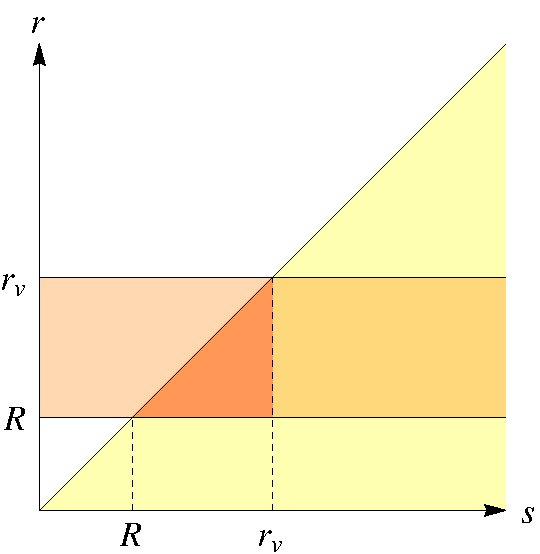
\includegraphics[width=0.5\linewidth]{domint}
	\caption{\footnotesize{}Le domaine d'intégration des différentes variables pour obtenir la dispersion de vitesse suivant la
	ligne de visée.}
	\label{fig:domint}
\end{figure}
Le domaine d'intégration global est celui qui est le mélange des couleurs en orange foncé et jaune foncé qui représentent la
subdivision de l'intégrale en deux domaines distincts qui vont faciliter la calcul de l'intégrale.

En décomposant l'intégrale suivant ces deux domaines et en développant l'expression, on obtient:
\begin{eqnarray}
        &&\Sigma{(R)}{\sigma_{LOS}}^2{(R)}=2\int_R^{r_v}{\frac{\pg{s+a}\pd}{s^2}{\nu(s)}{G}{M(s)}}{\dd{s}}\nonumber\\
        &\times&\pg\int_R^s{\pg\frac{r}{r+a}-\undemi\pg\frac{R}{r+a}\pd^2\pd\frac{1}{\sqrt{r^2-R^2}}\dd{r}}\pd\nonumber\\
        &+&2\int_{r_v}^{\infty}{\frac{\pg{s+a}\pd}{s^2}{\nu(s)}{G}{M(s)}}{\dd{s}}\nonumber\\
        &\times&\pg\int_R^{r_v}{\pg\frac{r}{r+a}-\undemi\pg\frac{R}{r+a}\pd^2\pd\frac{1}{\sqrt{r^2-R^2}}\dd{r}}\pd\nonumber\\
\end{eqnarray}
Si on récrit la densité surfacique comme (dimension variable selon les cas)
$\Sigma(R)=\frac{M(a)}{\pi{a^2}}\tilde{\Sigma}{(R/a,c)}=4{a}\nu(a)\tilde{\Sigma}{(R/a,c)}$, alors on peut aboutir en faisant le
calcul des intégrales à:
\begin{eqnarray}
        &&{\sigma_{LOS}}^2{(R)}={v_v}^2\frac{c/2}{\tilde{M}{(c)}\tilde{\Sigma}{(R/a,c)}}\nonumber\\
        &\times&\pg\int_{R/a}^c{{K}\pg{x\frac{a}{r},\frac{a}{r}}\pd}\tilde{\nu}{(x)}\frac{\tilde{M}{(x)}}{x}\dd{x}+I\pg{c\frac{a}{r},\frac{a}{r}}\pd{J(c)}\pd\nonumber\\
\end{eqnarray}
avec:
\small
\begin{eq}
        I(u,u_a)=\left\{\begin{array}{lr}
                                -u_a{\rm{sign}}(u_a-1)\frac{{u_a}^2-1/2}{|{u_a}^2-1|^{3/2}}{C^{-1}\pg\frac{1+u{u_a}}{u+u_a}\pd}&\\
                                \hspace{5em}+{\rm{acosh}}{u}+\frac{1/2}{u_a+u}\frac{\sqrt{u^2-1}}{{u_a}^2-1},&{u_a}\neq1\\
                                {\rm{acosh}}{u}-\sqrt{\frac{u-1}{u+1}}\pg\frac{8+7u}{6(1+u)}\pd,&{u_a}=1\\
                        \end{array}\right.
\end{eq}
\normalsize
\begin{eq}
        K(u,u_a)=\pg{1+\frac{u_a}{u}}\pd{I(u,u_a)}
\end{eq}
et:
\begin{eq}
        C^{-1}(X)=\left\{\begin{array}{lr}
                                {\rm{acosh}}{X}&u_a<1\\
                                {\rm{acos}}{X}&u_a>1\\
                         \end{array}\right.
\end{eq}
ainsi que:
\begin{eq}
        J(y)=\int_y^{\infty}\frac{x+1}{x^2}\tilde{\nu}{(x)}\tilde{M}{(x)}\dd{x}
\end{eq}
Cette dernière expression peut s'écrire également pour le modèle NFW:
\begin{eqnarray}
        &&J(y)=\frac{2}{3{y^2}(1+y)\pg\ln{4}-1\pd^2}\pg{y}\pg-3+y\pg-9+\pi^2\pg1+y\pd\pd\pd\right.\nonumber\\
        &&+3{y^3}\ln\pg1+\frac{1}{y}\pd+3\ln\pg1+y\pd\pg1-y+y^2\pg1+y\ln\pg1+y\pd\pd\pd\nonumber\\
        &&\left.-3{y^2}\ln\pg{y}\pg1+y\pd\pd+6{y^2}\pg1+y\pd{Li_2(-y)}\pd\nonumber\\
\end{eqnarray}
Donc finalement on peut rapidement et facilement calculer la dispersion de vitesse sur la ligne de visée pour vérifier si nos
modèles sont corrects pour être appliqués au calcul de la probabilité. Les premiers résultats étaient comme ceux décrits
précédemment, c'est-à-dire que le modèle ne collait pas parfaitement avec la dispersion de vitesse issue directement des données de
la simulation. Ceci était assez bizarre car dans \citet{MBM10} ce calcul avait été fait aussi et les résultats étaient assez
proches.

%Mais un jour la lumière a jailli et mis en évidence le fait que les calculs précédents utilisaient la concentration calculée à
%partir de la relation de \citet{MDvdB08} qui pour la masse virielle utilisée de \num{2e14}$M_{\odot}$ donne $\simeq$\num{5.8} et
%non pas une concentration de $c=4$ comme pour la simulation ce qui explique les écarts observés.

On peut maintenant tracer la dispersion de vitesse dans le cas de la simulation en gardant les particules dans le halo et avec une
coupure à \num{2.7}$\sigma_{LOS}{(R)}$. Les résultats sont sur la figure (\ref{fig:dispvitNFWcorr+27sig}).
\begin{figure}[htb]
	\centering
	\includegraphics[width=0.5\linewidth]{dispLOSEin+NFWcorr}
	\includegraphics[width=0.5\linewidth]{dispLOSEin+NFWcorr27sig}
	\caption{\footnotesize{}Graphe de la dispersion de vitesse calculée selon le modèle NFW en bleu et celle à partir des
	données de la simulation en rouge. En haut en prenant en compte les particules dans le halo et en bas en réalisant une
	coupure à \num{2.7}$\sigma_{LOS}{(R)}$.}
	\label{fig:dispvitNFWcorr+27sig}
\end{figure}
On voit alors que le modèle utilisé peut être difficilement mis en cause pour nos écarts dans la probabilité avec les données. Même
une fois la correction de la concentration apportée, des écarts existent toujours avec les contours de la probabilité hors on
discrimine un peu le modèle avec la dispersion de vitesse qui marche bien. On peut étayer cette remarque par la nouvelle densité de
particules dans les halos obtenue avec la concentration corrigée sur la figure (\ref{fig:ghcontcorr}).
\begin{figure}[htb]
	\centering
	\includegraphics[width=0.5\linewidth]{g_hContcorr}
	\caption{\footnotesize{}Nouveaux contours de la densité de particules dans les halos avec la concentration forcée cette
	fois à \num{4}.}
	\label{fig:ghcontcorr}
\end{figure}
Si les écarts observés avec la densité issue des données était la cause du problème, alors les résultats seraient inversés. En
effet le modèle sous-estime la vraie densité, donc $g_i/g_h$ est sur-estimé et alors la probabilité est sous-estimée. Or les
contours de la probabilité sont, comme on le voit sur la figure (\ref{fig:probcont}), au-dessus des contours de la simulation donc
le modèle sur-estime la probabilité pour les petits $R$ et les grands $v_z$. Le problème peut seulement venir alors de la densité des interlopers.
Cette densité est calculée pour une coupure à \num{2.7}$\sigma_{LOS}{(R)}$ pour le modèle et on voit sur la figure (\ref{fig:probcont})
que le modèle s'écarte des données au-dessus de cette coupure (la ligne verte sur le graphe) ce qui fait vraiment penser que le modèle
des interlopers est en cause car mal évalué au-dessus de cette coupure.
\begin{figure}[htb]
	\centering
	\includegraphics[width=0.5\linewidth]{ProbaCont}
	\caption{\footnotesize{}Contours de la probabilité issus des données en rouge, du modèle NFW en bleu et en vert la coupure
	à \num{2.7}$\sigma_{LOS}{(R)}$ de la vitesse suivant la ligne de visée.}
	\label{fig:probcont}
\end{figure}

Si le modèle des interlopers pose problème, il s'agit sans doute de la constante $B$ dans le modèle qui est mal évaluée. Elle
représente la composante plate de la densité dans le modèle mais on voit sur les graphes dans \citet{MBM10} que cette composante
fluctue assez au dessus de la coupure en vitesse sur la ligne de visée. Or c'est là que les probabilités calculées posent des
soucis. Donc il faut voir l'influence de ce paramètre sur notre estimation de la probabilité.

Le fait de faire varier cette composante plate a pu à certains endroits permettre de faire coïncider un peu mieux les contours bleu
et rouge, mais des fois accentue les écarts. En regardant \citet{MBM10}, on peut constater que sur les figures
(\ref{fig:interlopers}, pour des grands $v_z$ les fluctuations sont importantes et peuvent expliquer les différences observées
au-dessus de deux unités de vitesse virielle. Sauf à paramétrer cette constante avec le rayon projeté et la vitesse suivant la
ligne de visée, faire coïncider les données et le modèle est peine perdue. Il semble bien que dans cette région ce soit la densité
des interlopers qui impose ses règles pour la probabilité. Il faut donc prendre mieux en compte la densité des interlopers dans ce
domaine de l'espace des phases projeté pour avoir une bonne correspondance. Mais on peut s'interroger sur l'intérêt de réaliser ce
travail car les fluctuations observées dans la constante qui représente la composante plate de la densité des interlopers dépendent
essentiellement de la simulation utilisée et vont sûrement varier d'une simulation à l'autre. Ne traduisant pas une propriété
intrinsèque de la distribution des interlopers, ces fluctuations ne vont pas permettre de faire un meilleur calcul de la
probabilité quand on le réalisera en situation sur les données du SDSS, la distribution des interlopers fluctuant sûrement aussi
différemment dans ce domaine de l'espace des phases projeté.
\begin{figure}[htb]
	\centering
	\includegraphics[width=0.5\linewidth]{interlopers.png}
	\caption{\footnotesize{}Densité des interlopers en fonction de la vitesse suivant la ligne de visée. {\bfseries{a}}:
	dépendance avec le rayon projeté en bins croissants du rayon (rouge, vert, bleu, magenta, cyan). {\bfseries{b}}: dépendance
	en distance radiale. {\bfseries{c}}: dépendance en masse du halo. (voir l'article pour plus de précision)}
	\label{fig:interlopers}
\end{figure}

Il faut alors se résoudre (peut-être) à se limiter à ce calcul de la probabilité d'appartenance au halo au-dessus de la coupure en
vitesse de \num{2.7}$\sigma_{LOS}{(R)}$, au dessus la fluctuation de la densité des interlopers empêchant de réaliser un calcul
propre et précis.

Il s'avère que si on trace les contours de $g_h$ logarithmiquement, alors on voit que la densité de particules dans le halo du
modèle s'éloigne des données aux grandes vitesses suivant la ligne de visée (voir la figure (\ref{fig:ghcontlog})). Et ceci de
façon cohérente avec la surestimation expliquée plus haut. On ne peut plus incriminer la densité des interlopers mais bien la
densité des particules dans le halo.
\begin{figure}[htb]
	\centering
	\includegraphics[width=0.5\linewidth]{g_hContLog}
	\caption{\footnotesize{}Contours de la densité de particules dans le halo comme dans la figure mais les contours espacés
	logarithmiquement.}
	\label{fig:ghcontlog}
\end{figure}
Alors on peut se demander pourquoi la modélisation dans le cas du modèle ajusté directement ne marchait pas. Il est possible que
les particules qui sont près du centre soient problématiques dans la détermination des coefficients du modèle choisi. Selon les
recommandations de Gary, on va éliminer les particules en-dessous de \num{3}\% du rayon de viriel car la mauvaise détermination du
centre des halos peut influencer sur le choix du modèle qui colle le mieux aux données et faire croire que par exemple NFW est
meilleur que Einasto alors que non, et empêcher de trouver une modélisation.

\fs{Conclusion}
Durant le stage, plusieurs points importants pour aider à la réalisation de notre algorithme ont été mis en place. On a réalisé un
mock catalogue à partir des données de la simulation du Millennium-II qui nous permettra de tester les différents algorithmes
réalisés. Des caractéristiques comme une magnitude limite, correction-K ont été appliquées dessus afin de le faire correspondre au
mieux au SDSS.

L'algorithme de \citet{Yang+07} a été programmé pour avoir à notre disposition un algorithme de groupe qui pourra être comparé au
notre. Les différents outils utilisés pour y aboutir sont en place et pourront éventuellement être incorporés à notre algorithme
s'ils s'avèrent utiles (comme par exemple le FoF, ou la méthode de l'abundance matching). Les premiers résultats sont satisfaisant
à moitié, car il semble que le programme fonctionne bien pour certaines itérations et pas pour d'autres, la cause de ce problème
étant en cours de recherche.

Le principe de notre algorithme a aussi été discuté, et amélioré à partir des remarques sur les défauts que semble présenter sur
certains points l'algorithme de \citet{Yang+07}.

On estime que d'ici peu les deux algorithmes pourront fonctionner correctement et donner leur premier résultat sur le mock
catalogue et ensuite être appliqués sur le SDSS-DR7 afin de pouvoir comparer les résultats sur les groupes obtenus et leurs
propriétés.

Avec les améliorations que l'on apporte à notre algorithme par rapport à ceux déjà existants, les groupes devraient pouvoir être
mieux quantifiés ce qui devrait permettre d'avoir accès à une meilleure connaissance des effets de l'environnement des galaxies sur
leurs propriétés comme leur masse stellaire en fonction de la masse du halo, ou l'évolution de paramètres comme la métallicité avec
la position de la galaxie dans le groupe. Finalement, ces effets pourront alors être modélisés et intégrés sous forme de codes
semi-analytiques dans les simulations cosmologiques avec les modèles de formation de galaxies pour prendre mieux en compte la
physique de l'environnement, et réduire les écarts aux observations des données issues de ces simulations.

\scriptsize
Je tiens à remercier Thierry SOUSBIE pour ces conseils sur la réalisation d'un FoF "rapide" qui a permis de faciliter le travail
réalisé dans ce stage.
\normalsize
